% ### agregar ejemplos con dominios elementales y del teo. cambio de variable.
% ### agregar blabla.
% ### agregar ejemplos.
% ### corregir fubinis,2
% ### definir diam P

% ### definir set con big
% ### reescribir cuantificadores en inline math separados.
% ### \def'inir familia de elecci\'on.
% ### usar \: frente a \ref
% ### acortar demostraciones usando n\'umeros de ecuaciones y defs., aclarar demostraciones
% ### m parte de 1.
% ### cambiar abs por norm cuando corresponda
% ### cambiar | por abs
% corregir cdots, ldots por dotsc, dotsm, etc.
% req: uniforme continuidad, compactos.
% corregir (formalizar?) definiciones de integral de Riemann

%%%%%%%%%%%%%%%%%%%%%%%%

\chapter{Integraci\'on}\label{cap3}

%%%%%%%%%%%%%%%%%%%%%%%%

Nos interesa extender la noci\'on de ``\'area bajo una curva'', formalizada por la integral de Riemann en una variable, a la de ``\'area bajo una superficie'' en $\R^n $. Luego estudiaremos las propiedades fundamentales de la integral de Riemann en varias variables. Finalmente veremos algunas aplicaciones a problemas f\'isicos.

% \section{Algunas propiedades de la integral de Riemann en una
% variable que es imprescindible recordar}

% formula del cambio de variable
% tabla de primitivas usuales
% integraci\'on por partes

\section{Integral de Riemann en \texorpdfstring{$\R^2$}{R2}}\label{sec:RiemannR2}

\subsection{Definiciones}
\begin{definicion}
$R \subseteq \R^2 $ es un rect\'angulo\index{Rect\'angulo} \tssi{} $ R = [a_1, b_1] \times [a_2, b_2] $ con $ a_1,b_1,a_2,b_2 \in \R $.
\end{definicion}

El \'area de un rect\'angulo $ R = [a_1, b_1] \times [a_2, b_2] $ es
\[ V(R) = (b_1-a_1)(b_2-a_2) \]

\begin{definicion}
Para $m\in \N$, la $m$-equipartici\'on\index{m-equipartici\'on} del intervalo $ [a, b] $ con $ a,b \in \R $ es 
$$ \bigl\{[c_0, c_1], [c_1, c_2], \ldots,
[c_{m-1}, c_m]\bigr\} $$ 
con $ c_i = a + i\frac{b-a}{m}, i=0,
\ldots, m$. 
\end{definicion}
% La denotaremos $ \ep{m}{[a,b]} $. El largo de $ [a,b]
%$ es
%    \[ V([a,b]) = b-a \]
% \end{definicion}

\begin{figure}[H]
	\centering
	\input{figuras/equiparticion2.pdf_tex}
	\caption{2-equipartici\'on y selecci\'on}
\end{figure}

\begin{definicion}
Para $m\in \N$, la $m$-equipartici\'on del rect\'angulo $ R = [a_1, b_1] \times [a_2, b_2] $ es $ P = \{I_1 \times I_2 : I_i \in P_i, i=1, 2 \} $ con $ P_i $ $m$-equipartici\'on del intervalo $ [a_i, b_i] , i=1, 2 $. La denotaremos $ \ep{m}{R}$.
\end{definicion}

\begin{definicion}
Dado un rect\'angulo $ R \subseteq \R^2 $ y $m\in \N$, decimos que $ {(\vec{c}_P)}_{P \in \ep{m}{R}} $ es una \familiaEleccion{}\index{Selecci\'on} (para $\ep{m}{R}$) si $(\forall P \in \ep{m}{R}) \vec{c}_P \in P$.
\end{definicion}

Notar que cada elemento de una $m$-equipartici\'on es un rect\'angulo y que una $m$-equipartici\'on es finita, luego la siguiente definici\'on tiene sentido:

%\begin{definicion}
%Sea $ \emqc{m} $, $ R \subseteq \R^2 $ rect\'angulo, $ P_m $
%$m$-equipartici\'on de $ R $, $ f:R \to \R $ y una familia $
%{(\vec{c}_P)}_{P \in P_m}, \vec{c}_P \in P $. Se define la suma de Riemann
%asociada a $ m $, $ f $, y ${(\vec{c}_P)}_{P \in P_m} $ como:
%    \[S\left(f, {(\vec{c}_P)}_{P \in P_m}\right) = \sum_{P \in P_m} f(\vec{c}_P) V(P) \]
%\end{definicion}

\begin{definicion}
Sea $m\in \N$, $ R \subseteq \R^2 $ rect\'angulo, $ f:R \to \R$ y una \familiaEleccion{} $ {(\vec{c}_P)}_{P \in \ep{m}{R}} $. Se define la suma de Riemann \index{Suma!de Riemann} asociada a $ f $ y ${(\vec{c}_P)}_{P \in \ep{m}{R}} $ como:
\[S\left(f, {(\vec{c}_P)}_{P \in \ep{m}{R}}\right) = \sum_{P \in \ep{m}{R}} f(\vec{c}_P) V(P) \]
\end{definicion}

\begin{definicion}
%Sea $ R \subseteq \R^2 $ rect\'angulo, $ f:R \to \R $ acotada y,
%para $ \emqc{m} $, $P_m$ $m$-equipartici\'on de $R$. Entonces
%decimos que $f$ es Riemann integrable en $R$ \tssi{} $ (\exists S
%\in \R) $
%    \[ S = \lim_{m \to \infty} S\left(f, {(\vec{c}_P)}_{P \in P_m}\right) \]
%independiente de la elecci\'on de los $ {(\vec{c}_P)}_{P \in P_m} $.

Sea $ R \subseteq \R^2 $ rect\'angulo, $ f:R \to \R $. Decimos que $f$ es Riemann integrable \index{Funci\'on!Riemann integrable} en $R$ \tssi{} $ (\exists S \in \R) (\forall \varepsilon > 0) (\exists m_0\in \N) (\forall m \geq m_0)$
\[ \abs{ S\left(f, {(\vec{c}_P)}_{P \in \ep{m}{R}}\right) - S } < \varepsilon \]
para toda elecci\'on de los $ {(\vec{c}_P)}_{P \in \ep{m}{R}} $.

$S$ se llama integral (de Riemann) \index{Integral!de Riemann} de $f$ sobre $R$ y se denota:
\[ \int_R f \]
\end{definicion}

La integral de $f$ tambi\'en se anota:
\[ \int_R f(\vec{x})\,d\vec{x} \]

\begin{figure}[H]\label{fig:Riemann} 
   \centering
   \input{figuras/riemann.pdf_tex}
   \caption{Suma de Riemann para la funci\'on $f(x,y)=\sen\left(\frac{xy}{15}\right)$ para $ \ep{4}{[1,5]^2}$}
 \end{figure}

\begin{ejemplo}
Para $ R = [0,1]^2 $, no es integrable en $ R $ la funci\'on $ f : R\to \R $ dada por
    \[f(x,y) =
    \begin{cases}
        1& \text{ si } (x,y) \in \Q \times \Q \\
        0& \text{ si } (x,y) \notin \Q \times \Q
    \end{cases}
    \]
\end{ejemplo}

\subsection{Propiedades b\'asicas}

\begin{proposicion}
Sea $ R \subseteq \R^2 $ rect\'angulo, $ f:R \to \R $. Si $ f $ es integrable en $ R $ entonces $ f $ es acotada en $ R $.\index{Funci\'on!integrable}\index{Funci\'on!acotada}
\end{proposicion}

\begin{demostracion}
En efecto, sea $ \varepsilon = 1 $, $ m = m_0 $ en la definici\'on de integrabilidad. Luego
\begin{align*}
\abs{ S\left(f, {(\vec{c}_P)}_{P \in \ep{m}{R}}\right) - S } &< 1 \\
\babs{ \sum_{P \in \ep{m}{R}} f(\vec{c}_P) V(P) - S } 	   &< 1 \\
\babs{ \sum_{P \in \ep{m}{R}} f(\vec{c}_P) V(P) } 		   &< 1 + \abs{S}
\end{align*}
y para un cierto $ P_0 \in \ep{m}{R} $
\begin{align*}
    \bigabs{f(c_{P_0})} V(P_0) 						   &< 1 + \abs{S} +
    \babs{ \sum_{P \in \ep{m}{R} \setminus \{P_0\}} f(\vec{c}_P) V(P) } \\
\bigabs{f(c_{P_0})} 								   &< \frac{1}{V(P_0)}\biggl(1 + \abs{S} + \babs{
\sum_{P \in \ep{m}{R} \setminus \{P_0\}} f(\vec{c}_P) V(P) }\biggr)
\end{align*}
Fijando los $ \vec{c}_P$, para $P \in \ep{m}{R} \setminus \{P_0\} $ y notando que $ c_{P_0} $ es arbitrario en $ P_0 $ se concluye que $f $ es acotada en $ P_0 $. Como adem\'as $ P_0 $ es arbitrario en $\ep{m}{R} $ se concluye que $ f $ es acotada en cada $ P \in \ep{m}{R} $, luego $ f $ es acotada en $ R $.
\end{demostracion}

La siguiente propiedad es an\'aloga a la condici\'on de Cauchy para una sucesi\'on, luego es \'util por ejemplo para estudiar la integrabilidad de una funci\'on cuando no se conoce el valor de su integral.

\begin{proposicion}\label{pro:cauchy}
Sea $ R \subseteq \R^2 $ rect\'angulo, $ f:R \to \R $. Son equivalentes:
\begin{enumerate}
    \item $ \forall \varepsilon > 0, \exists m_0\in\N, \forall k, m
    \geq m_0, \forall \feleccion{{(\vec{c}'_P)}_{P \in \ep{k}{R}}}$,
    $\forall \feleccion{{(\vec{c}_P)}_{P \in \ep{m}{R}}} $
        \[ \abs{ S\left(f, {(\vec{c}'_P)}_{P \in \ep{k}{R}}\right) -
            S\left(f, {(\vec{c}_P)}_{P \in \ep{m}{R}}\right)} < \varepsilon \]
    \item $ f $ es integrable en $ R $.\index{Funci\'on!integrable}
\end{enumerate}
\end{proposicion}

\begin{demostracion}
\textcolor{white}{linea en blanco}
\\$(\Rightarrow)$: Fijemos ciertas \familiasEleccion{} ${(\vec{c}^m_P)}_{P \in \ep{m}{R}} $, para cada $m\in \N$. Luego, por la hip\'otesis, la sucesi\'on $${\left(S\left(f,{(\vec{c}^m_P)}_{P \in \ep{m}{R}}\right)\right)}_{m\in \N}$$ resulta ser de Cauchy y converge a un cierto $ S \in \R $. Sea $ \varepsilon> 0 $. Sea $ m_1 \geq m_0 $ tal que $ (\forall m \geq m_0) $
\[ \abs{ S\left(f,{(\vec{c}^m_P)}_{P \in \ep{m}{R}}\right) - S } < \varepsilon\]
Sea $ m \geq m_0 $ y una \familiaEleccion{} $ {(\vec{c}_P)}_{P \in \ep{m}{R}} $ arbitraria. As\'i, nuevamente con la hip\'otesis, resulta que
\begin{align*}
\abs{ S\left(f, {(\vec{c}_P)}_{P \in \ep{m}{R}}\right) - S }
    &\leq \abs{ S\left(f, {(\vec{c}_P)}_{P \in \ep{m}{R}}\right) -
        S\left(f,{(\vec{c}^{m_1}_P)}_{P \in P_{m_1}}\right) } \\
    &\quad + \abs{ S\left(f,{(\vec{c}^{m_1}_P)}_{P \in P_{m_1}}\right) - S } \\
    &< 2 \varepsilon
\end{align*}

\smallskip

$(\Leftarrow)$: Sea $ \varepsilon > 0 $, sea $m_0\in\N$ tal que $(\forall m \geq m_0)$
\[ \abs{ S\left(f, {(\vec{c}_P)}_{P \in \ep{m}{R}}\right) - S } < \varepsilon \]
para toda elecci\'on de los $ {(\vec{c}_P)}_{P \in \ep{m}{R}} $. Sean $ k,m \geq m_0 $ arbitrarios, sean $ {(\vec{c}_P)}_{P \in \ep{m}{R}}$, ${(\vec{c}'_P)}_{P \in \ep{k}{R}} $ \familiasEleccion{} arbitrarias.
Luego:
%\begin{multline*}
\begin{align*}
\abs{S\left(f,{(\vec{c}_P)}_{P \in \ep{m}{R}}\right) - S\left(f,{(\vec{c}'_P)}_{P \in
\ep{k}{R}}\right)}
%\begin{aligned}
    &\leq \abs{S\left(f,{(\vec{c}_P)}_{P \in \ep{m}{R}}\right) - S} \\
    &\quad + \abs{S - S\left(f,{(\vec{c}'_P)}_{P \in \ep{k}{R}}\right) } \\
    &\leq 2 \varepsilon
%\end{aligned}
%\end{multline*}
\end{align*}
\end{demostracion}

El siguiente lema es una consecuencia de la proposici\'on \ref{pro:cauchy} y nos da una condici\'on necesaria y suficiente de integrabilidad m\'as f\'acil de verificar en varias de las propiedades que siguen. La principal diferencia con la proposici\'on \ref{pro:cauchy} es que en vez de comparar todos los pares de particiones, compara pares de particiones que son una un refinamiento de la otra.

\begin{lema}\label{lem:Cauchy}
Sea $ R \subseteq \R^2 $ rect\'angulo, $ f:R \to \R $. Son equivalentes
\begin{enumerate}
    \item $ ( \forall \varepsilon > 0 )
        ( \exists m_0\in \N)
        ( \forall k\in \N)
        ( \forall m \geq m_0 )
        ( \forall \feleccion{{(\vec{c}_P)}_{P \in \ep{m}{R}}, {(\vec{c}'_P)}_{P \in
        \ep{km}{R}}} ) $
        \[ \sum_{P \in \ep{m}{R}}
            \sum_{\substack{Q \in \ep{km}{R} \\ Q \subseteq P}}
            \bigabs{ f(\vec{c}'_Q)-f(\vec{c}_P) } V(Q)
            < \varepsilon \]
    \item $ f $ es integrable en $ R $.\index{Funci\'on!integrable}
\end{enumerate}
\end{lema}

\begin{demostracion}
Usaremos la proposici\'on \ref{pro:cauchy} para sustituir la condici\'on $ f $ integrable en $ R $.

$(\Rightarrow)$: Sea $ \varepsilon > 0 $. Por hip\'otesis 
\[(\exists
 m_0\in \N) ( \forall  k\in \N)( \forall m \geq m_0 ) ( \forall
\feleccion{{(\vec{c}_P)}_{P \in \ep{m}{R}}} ) ( \forall
\feleccion{{(\vec{c}'_P)}_{P \in \ep{km}{R}}})
\]
\[    \sum_{P \in \ep{m}{R}} \sum_{\substack{Q \in \ep{km}{R} \\
    Q \subseteq P}} \bigabs{ f(\vec{c}'_Q)-f(\vec{c}_P) } V(Q)
            < \varepsilon 
\]
Sean $ k,m \geq m_0 $, sean $ {(\vec{c}_P)}_{P \in \ep{m}{R}}$, ${(\vec{c}'_P)}_{P \in \ep{k}{R}} $ \familiasEleccion{}. Sea ${(\vec{c}'_P)}_{P \in \ep{km}{R}} $ \familiaEleccion{}. Luego:
\begin{align*}
&\abs{S\left(f,{(\vec{c}'_Q)}_{Q \in \ep{km}{R}}\right) -
S\left(f,{(\vec{c}_P)}_{P \in \ep{m}{R}}\right)} \\
    &= \babs{ \sum_{Q \in \ep{km}{R}} f(\vec{c}'_Q) V(Q) -
        \sum_{P \in \ep{m}{R}} f(\vec{c}_P) V(P) } \\
    &= \babs{ \sum_{P \in \ep{m}{R}}
        \sum_{\substack{Q \in \ep{km}{R} \\ Q \subseteq P}} f(\vec{c}'_Q) V(Q) -
        \sum_{P \in \ep{m}{R}} f(\vec{c}_P)
        \sum_{\substack{Q \in \ep{km}{R} \\ Q \subseteq P}} V(Q) } \\
    &\leq \sum_{P \in \ep{m}{R}}
        \sum_{\substack{Q \in \ep{km}{R} \\ Q \subseteq P}}
        \bigabs{ f(\vec{c}'_Q)-f(\vec{c}_P) } V(Q) \\
    & < \varepsilon
\end{align*}
y an\'alogamente
\[
    \abs{S\left(f,{(\vec{c}'_Q)}_{Q \in \ep{km}{R}}\right) - S\left(f,{(\vec{c}'_P)}_{P \in
    \ep{k}{R}}\right)} < \varepsilon
\]
As\'i
%\begin{multline*}
\begin{align*}
&\abs{S\left(f,{(\vec{c}_P)}_{P \in \ep{m}{R}}\right) - S\left(f,{(\vec{c}'_P)}_{P \in \ep{k}{R}}\right)} \\
    &\leq \abs{S\left(f,{(\vec{c}_P)}_{P \in \ep{m}{R}}\right) - S\left(f,(\vec{c}'_Q)_{Q \in
    \ep{km}{R}}\right)} \\
    &\quad + \abs{S\left(f,(\vec{c}'_Q)_{Q \in \ep{km}{R}}\right) - S\left(f,{(\vec{c}'_P)}_{P \in \ep{k}{R}}\right) } \\
    &< 2 \varepsilon
\end{align*}
%\end{aligned}
%\end{multline*}

\smallskip

$(\Leftarrow)$: Sea $ \varepsilon > 0 $. Por hip\'otesis, $ ( \exists  m_0\in \N) ( \forall k, m \geq m_0 ) ( \forall \feleccion{{(\vec{c}'_P)}_{P \in \ep{k}{R}}}) (\forall \feleccion{{(\vec{c}_P)}_{P \in \ep{m}{R}}} ) $
\[ \abs{ S\left(f, {(\vec{c}'_P)}_{P \in \ep{k}{R}}\right) - S\left(f, {(\vec{c}_P)}_{P \in \ep{m}{R}}\right) } < \varepsilon \]
Sean $k\in \N$, $ m \geq m_0 $, sean ${(\vec{c}_P)}_{P \in \ep{m}{R}}, {(\vec{c}'_P)}_{P \in \ep{km}{R}}$ \familiasEleccion{}. Para $ P \in \ep{m}{R} $ definamos $$\vec{c}^+_P = \argmax \{f(\vec{c}'_Q):Q \in \ep{km}{R},Q \subseteq P\} \cup \{f(\vec{c}_P)\}$$ $$\vec{c}^-_P = \argmin \{f(\vec{c}'_Q):Q \in \ep{km}{R},Q \subseteq P\} \cup \{f(\vec{c}_P)\}$$
Luego
\begin{align*}
\sum_{P \in \ep{m}{R}} \sum_{\substack{Q \in \ep{km}{R} \\ Q
    \subseteq P}} &\bigabs{ f(\vec{c}'_Q)-f(\vec{c}_P) } V(Q) \\
& \leq \sum_{P \in \ep{m}{R}} \sum_{\substack{Q \in \ep{km}{R} \\
Q \subseteq P}} \bigl( f(\vec{c}^+_P)-f(\vec{c}^-_P) \bigr) V(Q) \\
& = \sum_{P \in \ep{m}{R}} \bigl( f(\vec{c}^+_P)-f(\vec{c}^-_P) \bigr) V(P) \\
& = S\left(f, {(\vec{c}^+_Q)}_{Q \in \ep{m}{R}}\right) - S\left(f,{(\vec{c}^-_P)}_{P \in \ep{m}{R}}\right) \\
&< \varepsilon
\end{align*}
\end{demostracion}

%\begin{proposicion}
%Sea $ R \subseteq \R^n $ rect\'angulo, $ f:R \to \R $. Si
%$ f $ es continua en $ R $ entonces $ f $ es uniformemente
%continua en $ R $.
%\end{proposicion}

% \begin{lema}
% Sea $ R \subseteq \R^n $ rect\'angulo, $ f:R \to \R $. Si $ f $
% es uniformemente continua en $ R $ entonces $ f $ es integrable
% en $ R $
% \end{lema}

Posteriormente (teorema \ref{teo:continuaEnCompactoEsuniformementeContinua}) probaremos que toda funci\'on continua sobre un rect\'angulo es uniformemente continua en \'el. En realidad lo probaremos para conjuntos mucho m\'as generales que rect\'angulos, llamados compactos. Esta propiedad se utiliza en la demostraci\'on de la siguiente proposici\'on.

\begin{proposicion}\label{pro:continua}
Sea $ R \subseteq \R^2 $ rect\'angulo, $ f:R \to \R $. Si $ f $ es continua en $ R $ entonces $ f $ es integrable en $ R $.\index{Funci\'on!integrable}
\end{proposicion}

%\begin{demostracion}
%Para $ \emqc{m} $, denotemos $ \ep{m}{R} $ la $m$-equipartici\'on de $ R
%$. Como $ R $ es compacto y $ f $ es continua en $ R $ se tiene
%que
%    %, por teorema  ###,
%$ f $ es uniformemente continua en $ R $.
%Luego, para $ \varepsilon > 0 $ arbitrario,  $ (\exists \delta >
%0)(\forall x,y \in R)$
%    \[ |x-y| < \delta \Rightarrow |f(x) - f(y)| < \varepsilon\]
%Sea $ \emqc{m_0} $ tal que $ (\forall P \in P_{m_0}\right)(\forall x,y
%\in P) |x-y| <
%\delta $. % Por ejemplo m_0>floor(diam(R)/delta
%Sean $ k,m \geq m_0 $, sean ${(\vec{c}'_P)}_{P \in \ep{k}{R}}$, ${(\vec{c}_P)}_{P \in
%\ep{m}{R}}$ dos \familiasEleccion{}. Probaremos que las sumas de
%Riemann asociadas se encuentran a distancia menor que $ \varepsilon
%$ por una constante, independiente de m, k y las familias.
%
%Sea $ {(\vec{c}'_P)}_{P \in \ep{km}{R}} $ \familiaEleccion{}. Luego:
%\begin{align*}
%\abs{S\left(f,{(\vec{c}_P)}_{P \in \ep{m}{R}}\right) - S\left(f,(c'_Q)_{Q \in \ep{km}{R}}\right)}
%    &= \abs{ \sum_{P \in \ep{m}{R}} f(\vec{c}_P) V(P) -
%        \sum_{Q \in \ep{km}{R}} f(\vec{c}'_Q) V(Q) } \\
%    &= \abs{ \sum_{P \in \ep{m}{R}} f(\vec{c}_P)
%        \sum_{\substack{Q \in \ep{km}{R} \\ Q \subseteq P}} V(Q) -
%        \sum_{P \in \ep{m}{R}}
%        \sum_{\substack{Q \in \ep{km}{R} \\ Q \subseteq P}} f(\vec{c}'_Q) V(Q) } \\
%    &\leq \sum_{P \in \ep{m}{R}}
%        \sum_{\substack{Q \in \ep{km}{R} \\ Q \subseteq P}}
%        \bigabs{ f(\vec{c}'_Q)-f(\vec{c}_P) } V(Q) \\
%\intertext{y con la uniforme continuidad}
%    & < \varepsilon V(R).
%\end{align*}
%As\'i
%\begin{align*}
%\abs{S\left(f,{(\vec{c}_P)}_{P \in \ep{m}{R}}\right) &- S\left(f,{(\vec{c}_P)}_{P \in \ep{k}{R}}\right)} \\
%    &\leq \abs{S\left(f,{(\vec{c}_P)}_{P \in \ep{m}{R}}\right) - S\left(f,(c'_Q)_{Q \in \ep{km}{R}}\right)}
%        + \abs{S\left(f,(c'_Q)_{Q \in \ep{km}{R}}\right) - S\left(f,{(\vec{c}_P)}_{P \in \ep{k}{R}}\right) } \\
%    &\leq 2 \varepsilon V(R).
%\end{align*}
%
%En particular, si fijamos las \familiasEleccion{} $ {(\vec{c}^*_P)}_{P
%\in \ep{m}{R}} $, la sucesi\'on $(S\left(f,{(\vec{c}^*_P)}_{P \in \ep{m}{R}}\right)_{\emqc{m}}$ es
%de Cauchy y converge a un cierto $ S \in \R $. En conclusi\'on,
%para $ m \geq m_0 $ y una \familiaEleccion{} arbitraria $
%{(\vec{c}^*_P)}_{P \in \ep{m}{R}} $ se tiene, escogiendo $ m_1 \geq m_0 $ tal
%que $ \abs{ S\left(f,{(\vec{c}^*_P)}_{P \in P_{m_1}}\right) - S } < \varepsilon $:
%\begin{align*}
%\abs{ S\left(f, {(\vec{c}_P)}_{P \in \ep{m}{R}}\right) - S }
%    &\leq \abs{ S\left(f, {(\vec{c}_P)}_{P \in \ep{m}{R}}\right) - S\left(f,{(\vec{c}^*_P)}_{P \in P_{m_1}}\right) } +
%        \abs{ S\left(f,{(\vec{c}^*_P)}_{P \in P_{m_1}}\right) - S } \\
%    &< \varepsilon (2 V(R) + 1)
%\end{align*}
%
%\end{demostracion}

\begin{demostracion}
Como $ R $ es compacto y $ f $ es continua en $ R $ se tiene que $ f $ es uniformemente continua en $ R $. Luego, para $ \varepsilon > 0 $ arbitrario,  $ (\exists \delta >0)(\forall \vec{x},\vec{y} \in R)$
\[ \norm{\vec{x}-\vec{y}} < \delta \Rightarrow \bigabs{f(\vec{x}) - f(\vec{y})} < \varepsilon\]
Recurriremos al lema \ref{lem:Cauchy}. Sea $m_0\in \N$ tal que $ (\forall P \in P_{m_0})(\forall \vec{x},\vec{y} \in P) \: \norm{\vec{x}-\vec{y}} < \delta $. 
% Por ejemplo m_0>floor(diam(R)/delta
Sea $ m \geq m_0 $, $k\in \N$. Sean ${(\vec{c}_P)}_{P \in \ep{m}{R}}$, $ {(\vec{c}'_P)}_{P \in \ep{km}{R}} $ \familiasEleccion{}.

Por la uniforme continuidad se tiene que
\[ \sum_{P \in \ep{m}{R}} \sum_{\substack{Q \in \ep{km}{R} \\ Q \subseteq P}} \bigabs{ f(\vec{c}'_Q)-f(\vec{c}_P) } V(Q) \leq \varepsilon V(R)\]
\end{demostracion}

\begin{proposicion}{\rm (Propiedades de la clase de funciones integrables)\index{Funciones integrables!propiedades}}
\\Sean $ R \subseteq \R^2 $ rect\'angulo, $f, g : R \to \R$ funciones integrables y $ c \in \R $. Se tienen las siguientes propiedades:
\begin{enumerate}
    \item Linealidad\index{Linealidad}: $f+cg$ es integrable en $ R $, entonces
        \[ \int_R f+cg = \int_R f + c \int_R g \]
    \item Monoton\'ia\index{Monoton\'ia}: si $(\forall x \in R) f(x) \leq g(x) $,
    entonces
        \[ \int_R f \leq \int_R g \]
    \item $ \abs{f} $ es integrable  en $ R $\index{Funci\'on!integrable en $R$}, entonces
        \[ \abs{ \int_R f } \leq \int_R \abs{f} \]
% formalizar disjunto salvo en los bordes?
%    \item (aditividad) si $ R_1, \ldots, R_k $ son rect\'angulos
%    disjuntos salvo en los bordes tales que $ R = \bigcup_{i=1}^k
%    R_i $, entonces
%        \[ \int_R f = \sum_{i=1}^k \int_{R_i} f \]
\end{enumerate}
\end{proposicion}

\begin{demostracion}
\begin{enumerate}
    \item Sea $ \varepsilon > 0 $ arbitrario. Sea $m_0\in \N$ tal
    que $ (\forall m \geq m_0)(\forall \feleccion{{(\vec{c}_P)}_{P \in \ep{m}{R}}} ) $
    \begin{align*}
        \abs{ S\left(f, {(\vec{c}_P)}_{P \in \ep{m}{R}}\right) - \int_R f } <
        \varepsilon \\
        \intertext{y}
        \abs{ S\left(g, {(\vec{c}_P)}_{P \in \ep{m}{R}}\right) - \int_R f } < \varepsilon
    \end{align*}
    Por otra parte, se tiene:
        \[ S\left(f+cg, {(\vec{c}_P)}_{P \in \ep{m}{R}}\right) = S\left(f, {(\vec{c}_P)}_{P \in \ep{m}{R}}\right)
        + cS\left(g, {(\vec{c}_P)}_{P \in \ep{m}{R}}\right)\]
    As\'i,
   % \begin{multline*}
    \begin{align*}
&    \abs{ S\left(f+cg, {(\vec{c}_P)}_{P \in \ep{m}{R}}\right) -
            (\int_R f + c \int_R g)} \\
%    \begin{aligned}
        &\leq \abs{ S\left(f, {(\vec{c}_P)}_{P \in \ep{m}{R}}\right) - \int_R f } +
            \abs{c} \abs{ S\left(g, {(\vec{c}_P)}_{P \in \ep{m}{R}}\right) - \int_R g } \\
        &\leq \bigl(1+\abs{c}\bigr) \varepsilon
 %   \end{aligned}
  %  \end{multline*}
\end{align*}
    Luego, por definici\'on de integral de Riemann, se concluye.
    \item Es directo de considerar que en este caso se cumple que
    $ \forall  m\in \N$, $\forall \feleccion{{(\vec{c}_P)}_{P \in \ep{m}{R}}}$
        \[ S\left(f, {(\vec{c}_P)}_{P \in \ep{m}{R}}\right) \leq S\left(g, {(\vec{c}_P)}_{P \in \ep{m}{R}}\right)
        \]
    y aplicar la definici\'on de integral de Riemann.
    \item Veamos que $ \abs{f} $ es integrable en $ R $ por medio
    del lema \ref{lem:Cauchy}.

    En
    efecto, sea $ \varepsilon > 0 $. Como $ f $ es integrable, por el mismo lema
    \\$( \exists  m_0\in \N) ( \forall  k\in \N)
        ( \forall m \geq m_0 )
        ( \forall \feleccion{{(\vec{c}_P)}_{P \in \ep{m}{R}}, {(\vec{c}'_P)}_{P \in \ep{km}{R}}} % ###
         ) $
        \[ \sum_{P \in \ep{m}{R}}
            \sum_{\substack{Q \in \ep{km}{R} \\ Q \subseteq P}}
            \bigabs{ f(\vec{c}'_Q)-f(\vec{c}_P) } V(Q)
        < \varepsilon \]
    Luego, sean $k\in \N $, $ m \geq m_0 $. Se sabe que $
    (\forall x,y \in \R) $
        \[ \bigabs{\abs{x} - \abs{y}} \leq \abs{x - y} \]
    As\'i
    \begin{align*}
        \sum_{P \in \ep{m}{R}}
            \sum_{\substack{Q \in \ep{km}{R} \\ Q \subseteq P}}
                &\bigabs{ \abs{f}(\vec{c}'_Q)-\abs{f}(\vec{c}_P) } V(Q) \\
        &\leq \sum_{P \in \ep{m}{R}}
            \sum_{\substack{Q \in \ep{km}{R} \\ Q \subseteq P}}
                \bigabs{ f(\vec{c}'_Q)-f(\vec{c}_P) } V(Q) \\
        &\leq \varepsilon
    \end{align*}
    En conclusi\'on, $ \abs{f} $ es integrable en $ R $. Finalmente,
    se tiene
        \[ -\abs{f} \leq f \leq \abs{f} \]
    que, con la parte anterior, implica que
        \[ -\int_R \abs{f} \leq \int_R f \leq \int_R \abs{f} \]
    es decir
        \[ \abs{ \int_R f } \leq \int_R \abs{f} \]
%    \item % ### preguntar que significa y hacer.
\end{enumerate}

\end{demostracion}

\begin{proposicion}\label{pro:estimacion}
Sea $ R \subseteq \R^2 $ rect\'angulo, $f : R \to \R$. Si $ f $ es
integrable en $ R $ entonces
    \[ V(R) \inf_{\vec{x} \in R} f(\vec{x}) \leq \int_R f \leq V(R) \sup_{\vec{x} \in R} f(\vec{x})\]
\end{proposicion}

\begin{demostracion}
Basta notar que $ \forall  m\in \N$, $\forall
\feleccion{{(\vec{c}_P)}_{P \in \ep{m}{R}}}$
    \[ V(R) \inf_{\vec{x} \in R} f(\vec{x})
        \leq S\left(f, {(\vec{c}_P)}_{P \in \ep{m}{R}}\right)
        \leq V(R) \sup_{\vec{x} \in R} f(\vec{x})\]
\end{demostracion}

\begin{figure}[H]\label{fig:cotaInferior} 
   \centering
   \input{figuras/cotainferior.pdf_tex}
   \caption{Ejemplo de que $V(R) \inf_{\vec{x} \in R} f(\vec{x}) \leq \int_R f $}
\end{figure}

\subsection{Integraci\'on de sucesiones de funciones\index{Integraci\'on!de sucesiones de funciones}}

\begin{proposicion}
Sea $ R \subseteq \R^2 $ rect\'angulo, ${(f_k)}_{k \in \N}$ sucesi\'on de funciones\index{Sucesi\'on!de funciones}, $f_k : R \to \R$, que convergen uniformemente en $ R $ a $ f: R \to \R $. Entonces $ f $ es integrable en $ R $\index{Funci\'on!integrable} y
    \[ \int_R f = \lim_{k \to \infty} \int_R f_k \]
\end{proposicion}

\begin{demostracion}
Veamos que $ f $ es integrable en $ R $ por medio del lema \ref{lem:Cauchy}. Sea $ \varepsilon > 0 $. Sea $k_0\in \N$ tal que
\begin{equation}\label{equ:f cerca fk0}
    \sup_{x \in R} \bigabs{ f(\vec{x}) - f_{k_0}(\vec{x}) } < \varepsilon 
\end{equation}
De acuerdo al lema \ref{lem:Cauchy}, sea $m_0\in \N$ tal que 
\\$( \forall k\in \N)( \forall m \geq m_0 ) ( \forall
\feleccion{{(\vec{c}_P)}_{P \in \ep{m}{R}},{(\vec{c}'_P)}_{P \in
\ep{km}{R}}} ) $
\begin{equation}\label{equ:fk0 integrable}
    \sum_{P \in \ep{m}{R}} \sum_{\substack{Q \in \ep{km}{R} \\ Q \subseteq P}}
        \bigabs{ f_{k_0}(\vec{c}'_Q)-f_{k_0}(\vec{c}_P) } V(Q) < \varepsilon 
\end{equation}

Luego, sean $k\in \N$, $ m \geq m_0 $. Por la desigualdad
triangular se tiene que
\begin{align*}
\sum_{P \in \ep{m}{R}} \sum_{\substack{Q \in \ep{km}{R} \\ Q
\subseteq P}}
        &\bigabs{ f(\vec{c}'_Q)-f(\vec{c}_P) } V(Q)\\
        &\leq \sum_{P \in \ep{m}{R}} \sum_{\substack{Q \in \ep{km}{R} \\ Q \subseteq
        P}}  \bigabs{ f(\vec{c}'_Q)-f_{k_0}(c'_Q) } V(Q) \\
    &\quad + \sum_{P \in \ep{m}{R}} \sum_{\substack{Q \in \ep{km}{R} \\ Q \subseteq
        P}} \bigabs{ f_{k_0}(c'_Q)-f_{k_0}(\vec{c}_P) } V(Q) \\
    &\quad + \sum_{P \in \ep{m}{R}} \sum_{\substack{Q \in \ep{km}{R} \\ Q \subseteq
        P}} \bigabs{ f_{k_0}(\vec{c}_P)-f(\vec{c}_P) } V(Q) \\
\intertext{y aplicando \ref{equ:f cerca fk0} y \ref{equ:fk0
integrable} se obtiene}
    &\leq \varepsilon \bigl( 2 V(R) + 1 \bigr)
\end{align*}
En conclusi\'on, $ f $ es integrable en $ R $. Por otra parte, por la proposici\'on \ref{pro:estimacion}
\begin{align*}
    \abs{ \int_R f_k - \int_R f }
        &= \abs{ \int_R (f_k - f) } \\
        &\leq \int_R \abs{f_k - f} \\
        &\leq V(R) \sup_{x \in R} \abs{ f_k(x) - f(x) }
\end{align*}
lo cual implica que
    \[ \int_R f = \lim_{k \to \infty} \int_R f_k \]
\end{demostracion}

\begin{ejemplo}
Una sucesi\'on de funciones integrables que converge puntualmente a un l\'imite que no lo es. Sea la numeraci\'on $ \{ q_0, q_1, \dotsc \} = [0, 1] \cap \Q $, sea $ I = [0,1] $ y las funciones $ f,f_n:I \to \R $ dadas por
\begin{align*}
f_n(\vec{x}) &=
    \begin{cases}
        1& \text{ si }(x,y) \in \{q_1, \dotsc, q_n\}\\
        0& \text{ si }(x,y) \notin \{q_1, \dotsc, q_n\}
    \end{cases} \\
f(\vec{x}) &=
    \begin{cases}
        1& (x,y) \in [0, 1] \cap \Q \\
        0& (x,y) \notin [0, 1] \cap \Q
    \end{cases}
\end{align*}
En $ I $, se tiene que $ f_n $ converge a $ f $ puntualmente (pero
no uniformemente) y cada $f_n$ es integrable, pero $ f $ no es
integrable.
\end{ejemplo}

\subsection{Extensi\'on de la clase de funciones integrables\index{Extensi\'on!de la clase de!funciones integrables}}

A\'un cuando la clase de funciones continuas es muy amplia, todav\'ia no es suficiente para muchas aplicaciones. As\'i, a continuaci\'on veremos una condici\'on suficiente de integrabilidad un poco m\'as d\'ebil que la continuidad, esto es, que una funci\'on sea continua salvo sobre la uni\'on de grafos de funciones continuas.

Recordar que el grafo de una funci\'on $ g: [a,b] \to \R $ es
\[ \grafo(g) = \bigr\{ (x,g(x)) \in \R^2 :  x \in [a,b]\bigr\} \]

Intuitivamente, el lema siguiente nos dice que el grafo de una funci\'on continua tiene ``volumen cero''.

\begin{lema}\label{lem:volumencero}
Sea  $ f: [a,b] \to [c,d] $ continua. Denotemos $ R = [a,b] \times
[c,d] $. Entonces
    \[ \lim_{m \to \infty} \sum_{\substack{P \in \ep{m}{R} \\ P \cap
    \grafo(g) \neq \varnothing}} V(P) = 0 \]
\end{lema}

\begin{demostracion}
Sea $\varepsilon > 0 $. Como $ f $ continua en $ [a,b] $ compacto, se tiene que $ f $ es uniformemente continua en $ [a,b] $ (teorema \ref{teo:continuaEnCompactoEsuniformementeContinua}). Luego $ (\exists \delta > 0) (\forall x,y \in [a,b]) $
\[ \abs{x-y}<\delta \Rightarrow \bigabs{f(x)-f(y)} < \varepsilon \]
As\'i, escojamos $m_0\in \N$ tal que $ (b-a)(d-c)/m_0 \leq \varepsilon $ y
\begin{equation}\label{equ:volumencero:cota}
    (b-a)/m_0 < \delta
\end{equation}
Entonces, se cumple que $ (\forall m \geq m_0 ) $
\begin{align*}
\sum_{\substack{P \in \ep{m}{R} \\ P \cap \grafo(g) \neq
\varnothing}} V(P)
    &= \frac{(b-a)(d-c)}{m^2} \card{\{ P \in \ep{m}{R} : P \cap
    \grafo(g) \neq \varnothing \}}
\end{align*}
Gracias a la uniforme continuidad y (\ref{equ:volumencero:cota})
\[
\card{\{ P \in \ep{m}{R} : P \cap \grafo(g) \neq \varnothing \}}
\leq m (\frac{\varepsilon}{(d-c)/m} + 1)
\] % ### oscuro
As\'i, $ \forall m \geq m_0 $
\begin{align*}
\sum_{\substack{P \in \ep{m}{R} \\ P \cap \grafo(g) \neq
\varnothing}} V(P)
    &\leq \frac{(b-a)(d-c)}{m^2} m (\frac{\varepsilon}{(d-c)/m} + 1) \\
    &= \varepsilon (b-a) + \frac{(b-a)(d-c)}{m} \\
    &\leq \varepsilon (b-a +1)
\end{align*}

\end{demostracion}

Para $ A \subseteq \R^n $ acotado, se define el di\'ametro de $ A $ como
\[\diam A = \sup_{x,y \in A} \norm{\vec{x}-\vec{y}}\]
\begin{figure}[H]
	\centering
	\input{figuras/diametro.pdf_tex}
	\caption{Di\'ametro de un conjunto $ A \subseteq \R^2 $}
\end{figure}

\begin{proposicion}
Sea $ R = [a,b] \times [c,d] \subseteq \R^2 $ rect\'angulo, $ f:R
\to \R $ acotada en $ R $ y continua en $ R \rightarrow \grafo(g) $,
donde $ g: [a,b] \to [c,d] $ es una funci\'on continua. Entonces $ f
$ es integrable en $ R $.\index{Funci\'on!integrable}
\end{proposicion}

\begin{demostracion}
Sea $ K \in \R $ tal que $ ( \forall x \in R ) $
\begin{equation}\label{equ:cota}
    \bigabs{f(\vec{x})} \leq K
\end{equation}
Recurriremos al lema \ref{lem:Cauchy}. Sea $ \varepsilon
> 0 $ arbitrario. De acuerdo al lema \ref{lem:volumencero}, sea $
m_0\in \N $ tal que $ (\forall m \geq m_0) $
\begin{equation}\label{equ:volumen:cero}
    \sum_{\substack{P \in \ep{m}{R} \\ P \cap
    \grafo(g) \neq \varnothing}} V(P) \leq \varepsilon
\end{equation}
Denotemos $ P^*_m = \{ P \in \ep{m}{R} : P \cap \grafo(g) =
\varnothing \} $, $ R_m^* = \bigcup_{P \in P^*_m} P $. Como $
R_{m_0}^* $ es compacto y $ f $ es continua en $ R_{m_0}^* $ se
tiene que
    %, por teorema  ###,
$ f $ es uniformemente continua en $ R_{m_0}^* $. Luego $ (\exists
\delta > 0)(\forall \vec{x},\vec{y} \in R_{m_0}^*)$
\begin{equation}\label{equ:unif:continuidad}
\|\vec{x}-\vec{y}\| < \delta \Rightarrow |f(x) - f(y)| < \varepsilon
\end{equation}
Sea $ m_1 \geq m_0 $ tal que $ (\forall P \in
\ep{m_1}{R})\diam{P} < \delta $. % Por ejemplo m_1>floor(diam(R)/delta
Sea $ m \geq m_1 $, $k\in \N$. Sean ${(\vec{c}_P)}_{P \in
\ep{m}{R}}$, $ {(\vec{c}'_P)}_{P \in \ep{km}{R}} $ \familiasEleccion{}.
As\'i
%\begin{align*}
%    \sum_{P \in \ep{m}{R}} &\sum_{\substack{Q \in \ep{km}{R} \\ Q \subseteq P}}
%        \bigabs{ f(\vec{c}'_Q)-f(\vec{c}_P) } V(Q) \\
%    &= \sum_{P \in P^*_m}
%        \sum_{\substack{Q \in \ep{km}{R} \\ Q \subseteq P}}
%        \bigabs{ f(\vec{c}'_Q)-f(\vec{c}_P) } V(Q) \\
%        &\quad + \sum_{P \in \ep{m}{R} \Rightarrow P^*_m}
%        \sum_{\substack{Q \in \ep{km}{R} \\ Q \subseteq P}}
%        \bigabs{ f(\vec{c}'_Q)-f(\vec{c}_P) } V(Q) \\
%\intertext{que, con \ref{equ:unif:continuidad}, implica que}
%    &\leq \varepsilon V(R) +
%        \sum_{P \in \ep{m}{R} \Rightarrow P^*_m}
%        \sum_{\substack{Q \in \ep{km}{R} \\ Q \subseteq P}}
%        \bigabs{ f(\vec{c}'_Q)-f(\vec{c}_P) } V(Q) \\
%\intertext{y con \ref{equ:cota} y \ref{equ:volumen:cero} resulta}
%    &\leq \varepsilon V(R) + \varepsilon 2K.
%\end{align*}
\begin{align*}
    \sum_{P \in \ep{m}{R}} &\sum_{\substack{Q \in \ep{km}{R} \\ Q \subseteq P}}
        \bigabs{ f(\vec{c}'_Q)-f(\vec{c}_P) } V(Q) \\
    &= \sum_{\substack{P \in \ep{m}{R} \\ P \subseteq R_{m_0}^*}}
        \sum_{\substack{Q \in \ep{km}{R} \\ Q \subseteq P}}
        \bigabs{ f(\vec{c}'_Q)-f(\vec{c}_P) } V(Q) + \sum_{\substack{P \in \ep{m}{R} \\ P \nsubseteq R_{m_0}^*}}
        \sum_{\substack{Q \in \ep{km}{R} \\ Q \subseteq P}}
        \bigabs{ f(\vec{c}'_Q)-f(\vec{c}_P) } V(Q) \\
\intertext{que, con (\ref{equ:cota}) y (\ref{equ:unif:continuidad}),
implica que}
    &\leq \varepsilon V(R) +
        2 K \sum_{\substack{P \in \ep{m}{R} \\ P \nsubseteq R_{m_0}^*}}
        V(P) \\
\intertext{y con (\ref{equ:volumen:cero}) resulta}
    &\leq \varepsilon V(R) + \varepsilon 18K % ### muy oscuro:argumento: rodear cada cuadradito que
    % toca el grafo con sus 8 vecinos = 9 cuadraditos.
\end{align*}
\end{demostracion}

\begin{corolario}
Sea $ R = [a,b] \times [c,d] \subseteq \R^2 $ rect\'angulo, $ f:R
\to \R $ acotada en $ R $ y continua en $ R \rightarrow
\bigcup_{i=1}^n\grafo(g_i) $, donde $ g_i: [a,b] \to [c,d] $ es
continua. Entonces $ f $ es integrable en $ R $.\index{Funci\'on!integrable}
\end{corolario}

\subsection{Teorema de Fubini}

El siguiente teorema expresa la integral de una funci\'on en 2 variables como la aplicaci\'on iterada de 2 integrales en una variable bajo hip\'otesis m\'inimas y permite escoger arbitrariamente el orden de estas integrales en una variable cuando la funci\'on a integrar es continua.

La demostraci\'on la haremos en la secci\'on \ref{sec:RiemannRN} en $\R^n $.

%\begin{lema}\label{lem:aditividad}
%Sean $ R \subseteq \R^2 $ rect\'angulo, $ f:R \to \R $, $
%\emqc{m^*} $. Si $ f $ es integrable en $ R $ entonces $ (\forall
%P \in \ep{m^*}{R} )$ $ f $ es integrable en $ P $ y
%    \[ \int_R f = \sum_{P \in \ep{m^*}{R}} \int_P f \]
%\end{lema}
%
%\begin{demostracion}
%Usaremos el lema \ref{lem:Cauchy}. Sean $\emqc{m^*} $, $
%\varepsilon > 0 $. Como $ f $ es integrable en $ R $, se tiene que $
%( \exists \emqc{m_0}\right) ( \forall \emqc{k}\right)( \forall m \geq m_0 ) (
%\forall \feleccion{{(\vec{c}_P)}_{P \in \ep{m}{R}}, {(\vec{c}_P)}_{P \in
%\ep{km}{R}}} ) $
%    \[ \sum_{P \in \ep{m}{R}}
%        \sum_{\substack{Q \in \ep{km}{R} \\ Q \subseteq P}}
%        \bigabs{ f(\vec{c}'_Q)-f(\vec{c}_P) } V(Q)
%    < \varepsilon \]
%Sean $ m \geq m_0 $, $ \emqc{k} $. As\'i, notando que $ \ep{mm^*}{R}
%= \biguplus_{S \in \ep{m^*}{R}} \ep{m}{S} $ obtenemos que
%\[
%    \sum_{S \in \ep{m^*}{R}}
%    \sum_{P \in \ep{m}{S}}
%    \sum_{\substack{Q \in \ep{km}{R} \\ Q \subseteq P}}
%    \bigabs{ f(\vec{c}'_Q)-f(\vec{c}_P) } V(Q)
%    < \varepsilon .
%\]
%En particular, $ (\forall S \in \ep{m^*}{R}\right) $
%\[
%    \sum_{P \in \ep{m}{S}}
%    \sum_{\substack{Q \in \ep{km}{R} \\ Q \subseteq P}}
%    \bigabs{ f(\vec{c}'_Q)-f(\vec{c}_P) } V(Q)
%    < \varepsilon .
%\]
%Es decir, $ (\forall S \in \ep{m^*}{R}\right) f $ es integrable en $ S
%$.
%
%Para concluir, la igualdad a probar es evidente de considerar la
%siguiente:
%    \[ S\left(f, {(\vec{c}_P)}_{P \in \ep{km^*}{R}}\right) = \sum_{S \in \ep{m^*}{R}} S\left(f,
%    {(\vec{c}_P)}_{P \in \ep{k}{S}}\right) \]
%\end{demostracion}

%\begin{lema}\label{lem:estimacion2}
%Sea $ R \subseteq \R^2 $ rect\'angulo, $f : R \to \R$, $
%\emqc{m^*} $. Si $ f $ es integrable en $ R $ entonces
%    \[ \sum_{S \in \ep{m^*}{R}} V(S) \inf_{x \in S} f(x) \leq \int_R f \leq
%    \sum_{S \in \ep{m^*}{R}} V(S) \sup_{x \in S} f(x)\]
%
%\end{lema}

%\begin{demostracion}
%En efecto, se tiene por el lema \ref{lem:aditividad} que
%    \[ \int_R f = \sum_{ S \in \ep{m^*}{R} } \int_S f \]
%Esto \'ultimo con la proposici\'on \ref{pro:estimacion} implica
%\[ \sum_{S \in \ep{m^*}{R}} V(S) \inf_{x \in S} f(x) \leq \int_R f \leq
%    \sum_{S \in \ep{m^*}{R}} V(S) \sup_{x \in S} f(x)\]
%\end{demostracion}

%\begin{demostracion}
%En efecto, es claro que $ \forall x \in R $
%\[
%    \sum_{S \in \ep{m^*}{R}} \ind{S}(x) \inf_{x \in S} f(x) \leq f(x)
%        \leq \sum_{S \in \ep{m^*}{R}} \ind{S}(x) \sup_{x \in S} f(x).
%\]
%Integrando se concluye la desigualdad buscada, notando que para $
%S \in \ep{m^*}{R} $ se tiene
%\[
%    \int_R \ind{S} = \int_S 1 = V(S).
%\]
%
%\end{demostracion}

 

\begin{teorema}{\rm (Teorema de Fubini en $\R^2$)\index{Teorema!de Fubini en $\R^2$}}\label{teo:FubiniR2}

Sea $ R = [a, b] \times [c, d] \subseteq \R^2 $ rect\'angulo, $f: R
\to \R$.
\begin{enumerate}
    \item Si $ f $ integrable en $ R $ y $ (\forall x \in [a, b])
    \:f(x, \cdot) $ integrable en $ [c, d] $, entonces
        \[ \int_R f = \int_a^b\left(\int_c^d f(x,y) \, dy\right)\, dx\]
    \item Si $ f $ continua en $ R $, entonces
        \[ \int_R f = \int_a^b\left(\int_c^d f(x,y)\,dy\right)\,dx
        = \int_c^d\left(\int_a^b f(x,y)\,dx\right)\,dy \]
\end{enumerate}
\end{teorema}

%\begin{demostracion}
%La segunda parte es consecuencia directa de la primera, en virtud
%de la proposici\'on \ref{pro:continua}. Probemos la primera parte.
%
%Definamos $ A = [a,b] $, $ B=[c,d] $, y la funci\'on $I:A \to \R $
%dada por $I(x) = \int_B f(x,y)dy $. Luego basta probar que $ I $
%es integrable en $ A $ y
%\[
%    \int_A I = \int_R f.
%\]
%
%En efecto, sea $ \varepsilon > 0 $ arbitrario. Por una parte, por
%definici\'on de integrabilidad, $ (\exists \emqc{m_0}\right) (\forall m
%\geq m_0)$
%\begin{equation}\label{equ:1}
%\babs{ \int_R f - \sum_{Q \in \ep{m}{R}} f(c_Q) V(Q) } < \varepsilon
%\end{equation}
%para toda elecci\'on de los $ {(\vec{c}_P)}_{P \in \ep{m}{R}} $.
%
%Por otra parte, sea $ m \geq m_0 $, $ (c_{Q_A}\right)_{Q_A \in
%\ep{m}a} $ \familiaEleccion{} arbitraria. Notar que
%\[
%    \ep{m}{R} = \bigl\{ Q_A \times Q_B :
%    Q_A \in \ep{m}a, Q_B \in \ep{m}{B} \bigr\}
%\]
%Consideremos la familia $ (c_Q^*)_{Q \in \ep{m}{R}} $ dada por
%(para $ Q_A \in \ep{m}a, Q_B \in \ep{m}{B} $) $ c_{Q_A \times
%Q_B}^* = ( c_{Q_A}, y^*) $, con $ y^* $ tal que $ f( c_{Q_A \times
%Q_B}^*) \geq \sup_{y \in Q_B} f( c_{Q_A}, y ) - \varepsilon $. As\'i,
%en virtud del lema \ref{lem:estimacion2} se tiene que
%\begin{align*}
%%\begin{multline*}
%    \sum_{Q_A \in \ep{m}a} I( c_{Q_A} ) &V(Q_A) - \sum_{Q \in
%        \ep{m}{R}} f( c_Q^* ) V(Q) \\
%%\begin{aligned}
%    &\leq \sum_{\substack{ Q_A \in \ep{m}a \\ Q_B \in \ep{m}{B} }}
%        \sup_{y \in Q_B} f(c_{Q_A}, y) V(Q_A)V(Q_B) \\
%    &\quad - \sum_{\substack{ Q_A \in \ep{m}a \\ Q_B \in \ep{m}{B} }}
%        f(c_{Q_A \times Q_B}^*) V(Q_A)V(Q_B) \\
%    &=  \sum_{\substack{ Q_A \in \ep{m}a \\ Q_B \in \ep{m}{B} }}
%        \bigl( \sup_{y \in Q_B} f(c_{Q_A},y) - f(c_{Q_A \times Q_B}^*) \bigr)
%        V(Q_A)V(Q_B) \\
%    &\leq \varepsilon V(R).
%%\end{aligned}
%%\end{multline*}
%\end{align*}
%An\'alogamente se obtiene que
%\[
%    -\varepsilon V(R) \leq
%        \sum_{Q_A \in \ep{m}a} I( c_{Q_A} ) V(Q_A) - \sum_{Q \in
%        \ep{m}{R}} f( c_Q^* ) V(Q)
%\]
%y, en conclusi\'on,
%
%\begin{equation}\label{equ:2}
%    \babs{ \sum_{Q_A \in \ep{m}a} I( c_{Q_A} ) V(Q_A) - \sum_{Q \in
%        \ep{m}{R}} f( c_Q^* ) V(Q) }
%    \leq \varepsilon V(R).
%\end{equation}
%Combinando \ref{equ:1} con \ref{equ:2} para la familia $
%(c_Q^*)_{Q \in \ep{m}{R}} $ se concluye que
%\[
%    \babs{ \sum_{Q_A \in \ep{m}a} I( c_{Q_A} ) V(Q_A) -
%        \int_R f }
%    \leq \varepsilon \bigl(V(R) + 1\bigr).
%\]
%
%\end{demostracion}

\begin{ejemplo}
Para $ R = [0,1] \times [0,1] $, calcular
\[
    \int_R x^2 + y
\]
\begin{solucion}
Por el teorema de Fubini, caso continuo, se tiene que
\begin{align*}
    \int_R x^2 + y &= \int_0^1 \left(\int_0^1 x^2 + y \,dy\right) \,dx \\
        &= \int_0^1 \left(x^2 y + \frac{y^2}{2} \evaluado_{y=0}^1\right)\,dx \\
        &= \int_0^1 x^2 + \frac{1}{2} \, dx \\
        &= \frac{x^3}{3} + \frac{x}{2} \evaluado_0^1 = \frac{5}{6}
\end{align*}
\end{solucion}
\end{ejemplo}

\begin{ejemplo}\label{ej:ejemploRaroFubini}
Veamos un caso en el que las integrales iteradas existen y son
iguales, pero la funci\'on no es integrable.

Consideremos el cuadrado unitario $ R = [0,1]^2 \subseteq \R^2 $ y la sucesi\'on de cuadrados $(R_k)_{k\in \N} $ contenidos en \'el dada por la figura \ref{fig:GraficoFubini1}. Dividamos cada $R_k $ en 4 cuadrados iguales $ R_k^{(1)}, R_k^{(2)}, R_k^{(3)},R_k^{(4)} $. Definamos la funci\'on $ f:R \to \R $ dada por
\[
f(x,y) =
\begin{cases}
    \frac{1}{V(R_k)} & \text{ si } (x,y) \in \interior R_k^{(1)}
    \cup \interior R_k^{(3)} \\
    -\frac{1}{V(R_k)} & \text{ si } (x,y) \in \interior R_k^{(2)}
    \cup \interior R_k^{(4)} \\
    0 & \text{ en otro caso }
\end{cases}
\]
Para cada $ y \in [0,1] $ es claro que
\[
\int_0^1 f(x,y) \, dx = 0
\]
y an\'alogamente para cada $ x \in [0,1] $
\[
\int_0^1 f(x,y) \, dy = 0
\]
Luego, las integrales iteradas son ambas nulas, esto es:
\[
    \int_0^1 \int_0^1 f(x,y) \, dy \, dx
    = \int_0^1 \int_0^1 f(x,y) \, dx \, dy
    = 0.
\]
Para convencernos de que $ f $ no es integrable, es suficiente ver que $ \abs{f} $ no es integrable. En efecto, $ \abs{f} $ est\'a dada por
\[
\abs{f}(x,y) =
\begin{cases}
\frac{1}{V(R_k)} & \text{ si } (x,y) \in R_k \\
0 & \text{en otro caso}
\end{cases}
\]
Si $ \abs{f} $ fuera integrable, como los $R_k$ son disjuntos, se tendr\'ia que
\[
    \int_R \abs{f} = \sum_{k \in \N} \int_{R_k} \abs{f}
\]
pero
\[
    \int_{R_k} \abs{f} = 1
\]
con lo que $ \abs{f} $ no puede ser integrable en $ R $.
\end{ejemplo}

\begin{figure}[H]
\begin{minipage}[t]{.45\textwidth}
	\centering
	\input{figuras/ejemplorarofubini.pdf_tex}
	\caption{El dominio del ejemplo \ref{ej:ejemploRaroFubini}.}
\label{fig:GraficoFubini1}
\end{minipage}
\hfill
\begin{minipage}[t]{.45\textwidth}
	\centering
	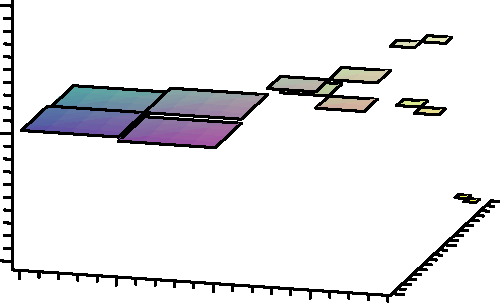
\includegraphics[width=\ScaleIfNeeded]{figuras/funcionejemplorarofubini.pdf}
	\caption{La funci\'on del ejemplo \ref{ej:ejemploRaroFubini}.}
\label{fig:GraficoFubini2}
\end{minipage}
\end{figure}


\subsection{Integral en \texorpdfstring{$\R^2$}{R2} sobre dominios generales \index{Integral!en $\R^2$ sobre dominios generales}}

A continuaci\'on extenderemos la definici\'on de integral para considerar la integraci\'on de funciones sobre algunos dominios un tanto m\'as generales que los rect\'angulos.
% definir indicatriz?
\begin{definicion} \label{def:IntegralSobreDominioGeneralR2}
Sea $ R \subseteq \R^2 $ rect\'angulo, $ A \subseteq R $, $f:A \to \R $. Denotemos $ f_0: R \to \R $ a la funci\'on dada por, para $x \in R $:
\[
    f_0(\vec{x}) = \begin{cases}
        f(\vec{x}) & \text{ si } \vec{x} \in A \\
        0    & \text{ si } \vec{x} \notin A
    \end{cases}
\]
Si $ f_0 $ es integrable sobre $ R $ entonces se dice que $ f $ es funci\'on integrable  \index{Funci\'on!integrable} sobre $ A $ y:
    \[ \int_A f = \int_R f_0 \]
\end{definicion}

\begin{definicion}
La funci\'on indicatriz\index{Funci\'on!indicatriz} de un conjunto $A\subseteq \R^2$ se define:
\[
    \ind{A}(\vec{x}) = \begin{cases}
        1	 & \text{ si } \vec{x} \in A \\
        0    & \text{ si } \vec{x} \notin A
    \end{cases}
\]
\end{definicion}

\begin{definicion}
Decimos que $ D \subseteq \R^2 $ es
\begin{enumerate}
    \item Dominio de tipo 1\index{Dominio!de tipo 1} \tssi{}
$\exists a,b \in \R$, $\exists \phi_1, \phi_2:[a,b] \to \R $
funciones continuas tales que $ (\forall x \in [a,b])\phi_1(x)
\leq \phi_2(x) $ y
    \[ D = \{(x,y) \in \R^2 : a \leq x \leq b, \phi_1(x)
    \leq y \leq \phi_2(x)\} \]
    \item Dominio de tipo 2\index{Dominio!de tipo 2} \tssi{} $\exists c,d
\in \R$, $\exists \psi_1, \psi_2:[c,d] \to \R $ funciones
continuas tales que $ (\forall x \in [c,d])\psi_1(x) \leq
\psi_2(x) $ y
    \[ D = \{(x,y) \in \R^2 : c \leq y \leq d, \psi_1(y)
    \leq x \leq \psi_2(y)\} \]
    \item Dominio de tipo 3\index{Dominio!de tipo 3} \tssi{} $ D $ es de tipo 1 y 2,
    \item Dominio elemental\index{Dominio!elemental} \tssi{} $ D $ es de tipo 1 \'o 2.
\end{enumerate}
\end{definicion}

\begin{figure}[htb]\label{fig:dominioTipo1y3}
	\begin{center}
	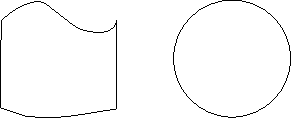
\includegraphics[scale=1.0]{figuras/dominioint.pdf}
	\end{center}
	\caption{Dominio del tipo 1 que no es del tipo 2 y dominio del
tipo 3.}
\end{figure}

% ### enmarcar y corregir lo de uni\'on finita de grafos de funciones.
Si $ R \subseteq \R^2 $ es un rect\'angulo y $ D \subseteq R $ es una regi\'on elemental entonces $ f_0 $ (dada por la definici\'on
\ref{def:IntegralSobreDominioGeneralR2}) es continua en $ R $ salvo sobre la uni\'on finita de grafos de funciones. Luego $ \int_D f $ existe. En general, supongamos que tenemos una funci\'on $ f: A \subseteq R \to \R $ con $ R $ rect\'angulo y $A$ dominio del tipo 1, digamos:
\[
    A = \{(x,y) \in \R^2 : a \leq x \leq b, \phi_1(x)
    \leq y \leq \phi_2(x)\}
\]
con $ a,b \in \R$, $ \phi_1, \phi_2:[a,b] \to \R $ funciones continuas. Entonces, gracias al teorema de Fubini (teorema \ref{teo:FubiniR2}), se tiene que:
\begin{align*}
    \int_A f = \int_a^b \int_{\phi_1(x)}^{\phi_2(x)} f(x,y) \, dy \,
    dx
\end{align*}

\begin{ejemplo}
Calcular
\[
    \int_T (x^3 y  + \cos(x)) \, dy \, dx
\]
donde
\[
    T = \{(x,y) \in \R^2 : 0 \leq x \leq \pi/2, 0 \leq y \leq x \}
\]
\begin{solucion}
Notar que $ T $ es una regi\'on del tipo 1. Por definici\'on se tiene
que
\begin{align*}
\int_T (x^3 y  + \cos(x)) \, dy \, dx
    &= \int_{[0,\pi/2]^2} \ind{T} (x^3 y  + \cos(x)) \, dy \, dx \\
\intertext{y, en virtud del teorema de Fubini:}
    &= \int_0^{\pi/2} \int_0^{\pi/2}
        \ind{T} \left(x^3 y  + \cos(x)\right) \, dy \, dx \\
\intertext{M\'as a\'un, con la definici\'on de $ T $:}
    &= \int_0^{\pi/2} \int_0^x \left(x^3 y  + \cos(x)\right) \, dy \, dx \\
    &= \int_0^{\pi/2} \left(\frac{x^3 y^2}{2} + y \cos(x)\right) \evaluado_{y=0}^x \, dx \\
    &= \int_0^{\pi/2} \frac{x^5}{2} + x \cos(x) \, dx \\
    &= \left( \frac{x^6}{12} + \cos(x) + x \sen(x)\right)\evaluado_0^{\pi/2} \\
    &= \frac{\pi^6}{768} + \frac{\pi}{2} - 1
\end{align*}
\end{solucion}
\end{ejemplo}
% ### hay otro ejemplo en el apunte.

\section{Integral de Riemann en \texorpdfstring{$\R^n$}{Rn}\index{Integral!de Riemann en $\R^n$}}\label{sec:RiemannRN}

Las demostraciones que no se incluyen en esta secci\'on son id\'enticas a las hechas en la secci\'on \ref{sec:RiemannR2}, acerca de la integral de Riemann en $ \R^2 $.

\subsection{Definiciones}

\begin{definicion}
$ R \subseteq \R^n $ es un rect\'angulo\index{Rect\'angulo} \tssi{} $ R = [a_1, b_1] \times \cdots \times [a_n, b_n] $ con $ a_i, b_i \in \R $.
\end{definicion}

\begin{definicion}
Para un rect\'angulo $ R = [a_1, b_1] \times \cdots \times [a_n, b_n] $ se define su volumen\index{Volumen!de un rect\'angulo} como
    \[ V(R) = \prod_{i=1}^n b_i-a_i \]
\end{definicion}

\begin{definicion}
Para $m\in \N$, la $m$-equipartici\'on\index{m-equipartici\'on} del rect\'angulo $ R = [a_1,b_1] \times \cdots \times [a_n, b_n] $ es $ \{I_1 \times \cdots \times I_n : I_i \in P_i, i=1, \ldots, n\} $ con $ P_i $ $m$-equipartici\'on del intervalo $ [a_i, b_i] , i=1, \ldots, n $. La denotaremos $ \ep{m}{R} $.
\end{definicion}

Dado un rect\'angulo $ R \subseteq \R^n $ y $m\in \N$, decimos que $ {(\vec{c}_P)}_{P \in \ep{m}{R}} $ es una \familiaEleccion{}\index{Selecci\'on} (para $ \ep{m}{R}$) si $(\forall P \in \ep{m}{R}) \vec{c}_P \in P $.

Notar que cada elemento de una $m$-equipartici\'on es un rect\'angulo y que una $m$-equipartici\'on es finita, luego la siguiente definici\'on tiene sentido:

\begin{definicion}
Sea $m\in \N$, $ R \subseteq \R^n $ rect\'angulo, $ f:R \to \R$ y una \familiaEleccion{} $ {(\vec{c}_P)}_{P \in \ep{m}{R}} $. Se define la suma de Riemann \index{Suma!de Riemann} asociada a $ f $ y ${(\vec{c}_P)}_{P \in \ep{m}{R}} $ como:
    \[S\left(f, {(\vec{c}_P)}_{P \in \ep{m}{R}}\right) = \sum_{P \in \ep{m}{R}} f(\vec{c}_P) V(P) \]
\end{definicion}

\begin{definicion}
Sea $ R \subseteq \R^n $ rect\'angulo, $ f:R \to \R $. Decimos que $f$ es Riemann integrable\index{Funci\'on!Riemann integrable} en $R$ \tssi{} $ (\exists S \in \R) $
    \[ \abs{ S\left(f, {(\vec{c}_P)}_{P \in \ep{m}{R}}\right) - S } < \varepsilon \]
para toda elecci\'on de los $ {(\vec{c}_P)}_{P \in \ep{m}{R}} $.

$S$ se llama integral (de Riemann) de $f$ sobre $R$ y se denota:
    \[ \int_R f \]
\end{definicion}

La integral de $f$ tambi\'en se anota:
    \[ \int_R f(\vec{x})\,d\vec{x} \]

\subsection{Propiedades B\'asicas \index{Integral!de Riemann en $\R^n$!Propiedades b\'asicas}}

%\begin{proposicion}
%Sea $ R \subseteq \R^n $ rect\'angulo, $ f:R \to \R $. Si
%$ f $ es continua en $ R $ entonces $ f $ es uniformemente
%continua en $ R $.
%\end{proposicion}

%\begin{lema}
%Sea $ R \subseteq \R^n $ rect\'angulo, $ f:R \to \R $. Si $ f $
%es uniformemente continua en $ R $ entonces $ f $ es integrable
%en $ R $
%\end{lema}

Las propiedades que enunciaremos tienen una demostraci\'on an\'aloga a las que ya vimos en el caso de $\R^2$.

\begin{proposicion}
Sea $ R \subseteq \R^n $ rect\'angulo, $ f:R \to \R $. Si $ f $ es integrable en $ R $ entonces $ f $ es acotada en $ R $\index{Funci\'on!acotada en $R$}.
\end{proposicion}

\begin{proposicion} %\label{pro:cauchy}
Sea $ R \subseteq \R^n $ rect\'angulo, $ f:R \to \R $. Son equivalentes:
\begin{enumerate}
    \item $ \forall \varepsilon > 0, \exists m_0\in \N\: \forall k, m
    \geq m_0, \forall \feleccion{{(\vec{c}'_P)}_{P \in \ep{k}{R}}} $,
    $\forall \feleccion{{(\vec{c}_P)}_{P \in \ep{m}{R}}}  $
        \[ \abs{ S\left(f, {(\vec{c}'_P)}_{P \in \ep{k}{R}}\right) -
            S\left(f, {(\vec{c}_P)}_{P \in \ep{m}{R}}\right) } < \varepsilon \]
    \item $ f $ es integrable en $ R $.\index{Funci\'on!integrable}
\end{enumerate}
\end{proposicion}

\begin{proposicion}
Sea $ R \subseteq \R^n $ rect\'angulo, $ f:R \to \R $. Si $ f $ es continua en $ R $ entonces $ f $ es integrable en $ R $.
\end{proposicion}

\begin{proposicion}
Sean $ R \subseteq \R^n $ rect\'angulo, $f, g : R \to \R$ funciones integrables \index{Funciones integrables} y $ c \in \R $. Se tienen las siguientes propiedades:
\begin{enumerate}
    \item Linealidad\index{Linealidad}: $f+cg$ es integrable, entonces
        \[ \int_R f+cg = \int_R f + c \int g \]
    \item Monoton\'ia\index{Monoton\'ia}: si $(\forall x \in R) f(x) \leq g(x) $, entonces
        \[ \int_R f \leq \int_R g \]
    \item $ \abs{f} $ es integrable en $ R $\index{Funci\'on!integrable en $R$}, entonces
        \[ \abs{ \int_R f } \leq \int_R \abs{f} \]
% formalizar disjuntos\ldots ?
%    \item (aditividad) si $ R_1, \ldots, R_k $ son rect\'angulos
%    disjuntos salvo en los bordes tales que $ R = \bigcup_{i=1}^k
%    R_i $, entonces $f$ integrable en $ R_i $ y
%        \[ \int_R f = \sum_{i=1}^k \int_{R_i} f \]
\end{enumerate}
\end{proposicion}

\begin{proposicion} %\label{pro:estimacion}
Sea $ R \subseteq \R^n $ rect\'angulo, $f : R \to \R$. Si $ f $ es integrable en $ R $ entonces
    \[ V(R) \inf_{\vec{x} \in R} f(\vec{x}) \leq \int_R f \leq V(R) \sup_{\vec{x} \in R} f(\vec{x})\]
\end{proposicion}

\subsection{Integraci\'on de sucesiones de funciones \index{Integraci\'on!de sucesiones de funciones}}

\begin{proposicion} \label{pro:convergencia}
Sea $ R \subseteq \R^n $ rect\'angulo, ${(f_k)}_{k \in \N}$ sucesi\'on de funciones, $f_k : R \to \R$, que convergen uniformemente en $ R $ a $ f: R \to \R $. Entonces $ f $ es integrable en $ R $\index{Funci\'on!integrable} y
    \[ \int_R f = \lim_{k \to \infty} \int_R f_k \]
\end{proposicion}

\subsection{Extensi\'on de la clase de funciones integrables\index{Extensi\'on!de la clase de!funciones integrables}}

Recordar que el grafo de una funci\'on $ g: A \subseteq \R^n \to
\R^m $ es
    \[ \grafo(g) = \{ (\vec{x},g(\vec{x})) \in \R^{n+m} :  \vec{x} \in A\} \]

La demostraci\'on del siguiente lema es an\'aloga a la del lema \ref{lem:volumencero}.

\begin{lema} %\label{lem:volumencero}
Sea  $ R' \subseteq \R^{N-1} $ rect\'angulo, $ f: R' \to [a,b] $
continua. Denotemos $ R = R' \times [a,b] $. Entonces
    \[ \lim_{m \to \infty} \sum_{\substack{P \in \ep{m}{R} \\ P \cap
    \grafo(g) \neq \varnothing}} V(P) = 0 \]
\end{lema}

\begin{demostracion}
Sea $\varepsilon > 0 $. Como $ f $ continua en $ R' $ compacto, se tiene que $ f $ es uniformemente continua en $ R' $. Luego $(\exists \delta > 0) (\forall \vec{x},\vec{y} \in R') $
    \[ \norm{\vec{x}-\vec{y}}<\delta \Rightarrow \bigabs{f(\vec{x})-f(\vec{y})} < \varepsilon \]
As\'i, escojamos $m_0\in \N$ tal que $ V(R)/m_0 \leq \varepsilon $ y $ \diam{P} < \delta $, para cualquier $ P \in \ep{m}{R'} $. Entonces, se cumple que $ (\forall m \geq m_0 ) $
\begin{align*}
\sum_{\substack{P \in \ep{m}{R} \\ P \cap \grafo(g) \neq
\varnothing}} V(P)
    &= \frac{V(R)}{m^N} \card{\{ P \in \ep{m}{R} : P \cap
    \grafo(g) \neq \varnothing \}} \\
    &\leq \frac{V(R)}{m^N} m^{N-1} (\frac{\varepsilon}{(b-a)/m} + 1) \\ % ### oscuro
    &= \varepsilon V(R') + \frac{V(R)}{m} \\
    &\leq \varepsilon (V(R') +1)
\end{align*}
\end{demostracion}

\begin{proposicion}
Sea $ R' \subseteq \R^{N-1}$ rect\'angulo, $ R = R' \times [a,b] \subseteq \R^n $ rec\-t\'an\-gu\-lo, $ f:R \to \R $ acotada en $R$ y continua en $ R \rightarrow \grafo(g) $, donde $ g: R' \to [a,b] $ es una funci\'on continua. Entonces $ f $ es integrable en $ R $.\index{Funci\'on!integrable}
\end{proposicion}

%\begin{proposicion}
%Sea $ R = [a,b] \times [c,d] \subseteq \R^2 $ rect\'angulo, $ f:R
%\to \R $ acotada y continua en $ R \backslash
%\bigcup_{i=1}^n\grafo(g_i) $, donde $ g_i: [a,b] \to [c,d] $ es
%una funci\'on continua. Entonces $ f $ es integrable en $ R $.
%\end{proposicion}

\begin{corolario}
Sea $ R' \subseteq \R^{N-1}$ rect\'angulo, $ R = R' \times [a,b] \subseteq \R^n $ rect\'angulo, $ f:R \to \R $ acotada en $ R $ y continua en $ R \rightarrow \bigcup_{i=1}^n\grafo(g_i) $, donde $ g_i: R' \to [a,b] $ es continua. Entonces $ f $ es integrable en $ R $.\index{Funci\'on!integrable}
\end{corolario}

\subsection{Teorema de Fubini}

\begin{lema}\label{lem:estimacion2}
Sea $ R \subseteq \R^n $ rect\'angulo, $f : R \to \R$, $m^*\in \N$. Si $ f $ es integrable en $ R $ entonces
    \[ \sum_{S \in \ep{m^*}{R}} V(S) \inf_{\vec{x} \in S} f(\vec{x}) \leq \int_R f \leq \sum_{S \in \ep{m^*}{R}} V(S) \sup_{\vec{x} \in S} f(\vec{x})\]
\end{lema}

%\begin{demostracion}
%En efecto, se tiene por el lema \ref{lem:aditividad} que
%    \[ \int_R f = \sum_{ S \in \ep{m^*}{R} } \int_S f \]
%Esto \'ultimo con la proposici\'on \ref{pro:estimacion} implica
%\[ \sum_{S \in \ep{m^*}{R}} V(S) \inf_{x \in S} f(x) \leq \int_R f \leq
%    \sum_{S \in \ep{m^*}{R}} V(S) \sup_{x \in S} f(x)\]
%\end{demostracion}

\begin{demostracion}
En efecto, es claro que $ \forall \vec{x} \in R $
\[
    \sum_{S \in \ep{m^*}{R}} \ind{S}(\vec{x}) \inf_{\vec{x} \in S} f(\vec{x}) \leq f(\vec{x})
        \leq \sum_{S \in \ep{m^*}{R}} \ind{S}(\vec{x}) \sup_{\vec{x} \in S} f(x).
\]
Integrando se concluye la desigualdad buscada, notando que para $S \in \ep{m^*}{R} $ se tiene
\[
    \int_R \ind{S} = \int_S 1 = V(S)
\]

\end{demostracion}

\begin{teorema}{\rm (Teorema de Fubini en $\R^n$\index{Teorema!de Fubini en $\R^n$})} \label{teo:FubiniRN}

Sean $M,N\in \N$, $ A \subseteq \R^n $, $ B \subseteq \R^m $ rect\'angulos, notemos $ R = A \times B \subseteq \R^{n+m} $ rect\'angulo. Sea $f: R \to \R$.
\begin{enumerate}
    \item Si $ f $ integrable en $ R $ y $ (\forall \vec{x} \in A)
    f(\vec{x}, \cdot) $ integrable en $ B $, entonces
        \[ \int_R f = \int_A\left(\int_B f(\vec{x},\vec{y}) \, d\vec{y}\right)\, d\vec{x}\]
    \item Si $ f $ continua en $ R $, entonces
        \[ \int_R f = \int_A\left(\int_B f(\vec{x},\vec{y})\,d\vec{y}\right)\,d\vec{x}
        = \int_B\left(\int_A f(\vec{x},\vec{y})\,d\vec{x}\right)\,d\vec{y} \]
\end{enumerate}
\end{teorema}
% ### rehacerlo en R^3, etc.

\begin{demostracion}
La segunda parte es consecuencia directa de la primera, en virtud de la proposici\'on \ref{pro:continua}. Probemos la primera parte.

Definamos la funci\'on $I:A \to \R $ dada por $I(x) = \int_B f(\vec{x},\vec{y})d\vec{y} $. Luego basta probar que $ I $ es integrable en $ A $ y
\[
    \int_A I = \int_R f
\]

En efecto, sea $ \varepsilon > 0 $ arbitrario. Por una parte, por definici\'on de integrabilidad, $(\exists m_0\in \N) (\forall m \geq m_0)$
\begin{equation}\label{equ:1}
\babs{ \int_R f - \sum_{Q \in \ep{m}{R}} f(\vec{c}_Q) V(Q) } < \varepsilon
\end{equation}
para toda elecci\'on de los $ {(\vec{c}_Q)}_{Q \in \ep{m}{R}} $.

Por otra parte, sea $ m \geq m_0 $, $ {(\vec{c}_{Q_A})}_{Q_A \in \ep{m}a} $ \familiaEleccion{} arbitraria. Notar que
\[
    \ep{m}{R} = \bigl\{ Q_A \times Q_B :
    Q_A \in \ep{m}a, Q_B \in \ep{m}{B} \bigr\}
\]
Consideremos la \familiaEleccion{} $ {(\vec{c}_Q^*)}_{Q \in \ep{m}{R}} $ dada por (para $ Q_A \in \ep{m}a, Q_B \in \ep{m}{B} $) $ \vec{c}_{Q_A \times Q_B}^* = ( \vec{c}_{Q_A}, y^*) $, con $ y^* $ tal que $ f( \vec{c}_{Q_A \times Q_B}^*) \geq \sup_{y \in Q_B} f( \vec{c}_{Q_A}, y ) - \varepsilon $.
As\'i, en virtud del lema \ref{lem:estimacion2} se tiene que
\begin{align*}
%\begin{multline*}
    \sum_{Q_A \in \ep{m}a} I( \vec{c}_{Q_A} ) &V(Q_A) - \sum_{Q \in
        \ep{m}{R}} f( \vec{c}_Q^* ) V(Q) \\
%\begin{aligned}
    &\leq \sum_{\substack{ Q_A \in \ep{m}a \\ Q_B \in \ep{m}{B} }}
        \sup_{\vec{y} \in Q_B} f(\vec{c}_{Q_A}, \vec{y}) V(Q_A)V(Q_B) \\
    &\quad - \sum_{\substack{ Q_A \in \ep{m}a \\ Q_B \in \ep{m}{B} }}
        f(c_{Q_A \times Q_B}^*) V(Q_A)V(Q_B) \\
    &=  \sum_{\substack{ Q_A \in \ep{m}a \\ Q_B \in \ep{m}{B} }}
        \bigl( \sup_{\vec{y} \in Q_B} f(\vec{c}_{Q_A},\vec{y}) - f(\vec{c}_{Q_A \times Q_B}^*) \bigr)
        V(Q_A)V(Q_B) \\
    &\leq \varepsilon V(R)
%\end{aligned}
%\end{multline*}
\end{align*}
Combinando con (\ref{equ:1}) se obtiene:
\begin{align*}
    \sum_{Q_A \in \ep{m}a} I( \vec{c}_{Q_A} ) V(Q_A) -
        \int_R f
    \leq \varepsilon \bigl(V(R) + 1\bigr)
\end{align*}
Escogiendo $ {(\vec{c}_Q^*)}_{Q \in \ep{m}{R}} $ tal que $ f( \vec{c}_{Q_A
\times Q_B}^*) \leq \inf_{\vec{y} \in Q_B} f( \vec{c}_{Q_A}, \vec{y} ) + \varepsilon $,
un c\'alculo an\'alogo permite obtener:
\begin{align*}
    - \varepsilon \bigl(V(R) + 1\bigr)
    \leq \sum_{Q_A \in \ep{m}a} I( \vec{c}_{Q_A} ) V(Q_A) -
        \int_R f
\end{align*}
En conclusi\'on,
\[
    \babs{ \sum_{Q_A \in \ep{m}a} I( \vec{c}_{Q_A} ) V(Q_A) -
        \int_R f }
    \leq \varepsilon \bigl(V(R) + 1\bigr)
\]

%An\'alogamente se obtiene que
%\[
%    -\varepsilon V(R) \leq
%        \sum_{Q_A \in \ep{m}a} I( c_{Q_A} ) V(Q_A) - \sum_{Q \in
%        \ep{m}{R}} f( c_Q^* ) V(Q)
%\]
%y, en conclusi\'on,
%
%\begin{equation}\label{equ:2}
%    \babs{ \sum_{Q_A \in \ep{m}a} I( c_{Q_A} ) V(Q_A) - \sum_{Q \in
%        \ep{m}{R}} f( c_Q^* ) V(Q) }
%    \leq \varepsilon V(R).
%\end{equation}
%Combinando \ref{equ:1} con \ref{equ:2} para la familia $
%{(c_Q^*)}_{Q \in \ep{m}{R}} $ se concluye que
%\[
%    \babs{ \sum_{Q_A \in \ep{m}a} I( c_{Q_A} ) V(Q_A) -
%        \int_R f }
%    \leq \varepsilon \bigl(V(R) + 1\bigr).
%\]
\end{demostracion}

\begin{ejemplo}
Calcular $ \int_B f$ con $ B = [0,1]^3 \times [0, 10] $ y $f(x,y,z,t) = t(x^2+y^2+z^2) $.

\begin{solucion}
En virtud del teorema de Fubini
\begin{align*}
\int_B f
    &= \int_0^{10} \int_0^1 \int_0^1 \int_0^1 t(x^2+y^2+z^2) \, dx
    \, dy \, dz \, dt \\
    &= \int_0^{10} \int_0^1 \int_0^1
        (t \frac{x^3}{3} + t y^2 x + t z^2 x) \evaluado_{x=0}^1
        \, dy \, dz \, dt\\
    &= \int_0^{10} \int_0^1 \int_0^1
        (\frac{t}{3} + t y^2 + t z^2) \, dy \, dz \, dt\\
    &= \int_0^{10} \int_0^1 (\frac{t}{3} y + t \frac{y^3}{3} + t z^2 y)
        \evaluado_{y=0}^1 \, dz \, dt \\
    &= \int_0^{10} \int_0^1 (\frac{t}{3} + \frac{t}{3} + t z^2)
        \, dz \, dt \\
    &= \int_0^{10} t \, dt \\
    &= 50.
\end{align*}
\end{solucion}
\end{ejemplo}

\subsection{Integral en \texorpdfstring{$\R^n$}{Rn} sobre dominios generales \index{Integral!en $\R^n$ sobre dominios generales}}
% ### permutar las 2 definiciones siguientes ?
\begin{definicion} \label{def:IntegralSobreDominioGeneralRN}
Sea $ R \subseteq \R^n $ rect\'angulo, $ A \subseteq R $, $f:A \to \R $. Denotemos $ f_0: R \to \R $ a la funci\'on dada por, para $ x \in R $:
\[
    f_0(\vec{x}) = \begin{cases}
        f(\vec{x}) & \text{ si } \vec{x} \in A \\
        0    & \text{ si } \vec{x} \notin A
    \end{cases}
\]
Si $ f_0 $ es integrable sobre $ R $ entonces se dice que $ f $ es integrable sobre $ A $ y:
    \[ \int_A f = \int_R f_0 \]
\end{definicion}

\begin{definicion}
La funci\'on indicatriz\index{Funci\'on!indicatriz} de un conjunto $A\subseteq \R^n$ es an\'aloga al caso de $\R^2$ y se define:
\[
    \ind{A}(\vec{x}) = \begin{cases}
        1	 & \text{ si } \vec{x} \in A \\
        0    & \text{ si } \vec{x} \notin A
    \end{cases}
\]
\end{definicion}

\begin{definicion}
Decimos que $ D \subseteq \R^3 $ es
\begin{enumerate}
    \item Dominio de tipo 1\index{Dominio!de tipo 1} \tssi{} alguna de las siguientes afirmaciones
    es cierta:
    \begin{enumerate}
        \item $\exists a,b \in \R$, $\exists \phi_1, \phi_2:[a,b] \to
\R $ funciones continuas, $\exists \gamma_1, \gamma_2:D' \to \R
$ funciones continuas tales que
\begin{align*}
    D = \{(x,y,z) \in \R^3 : a &\leq x \leq b, \\
    \phi_1(x) &\leq y \leq \phi_2(x), \\
    \gamma_1(x,y) &\leq z \leq \gamma_2(x,y)\}
\end{align*}
donde $ D' = \{(x,y) \in \R^2: a \leq x \leq b, \phi_1(x) \leq y
\leq \phi_2(x) \} $
        \item $\exists c,d \in \R$, $\exists \psi_1, \psi_2:[c,d] \to
\R $ funciones continuas, $\exists \gamma_1, \gamma_2:D' \to \R
$ funciones continuas tales que
\begin{align*}
    D = \{(x,y,z) \in \R^3 : c &\leq y \leq d, \\
    \psi_1(y) &\leq x \leq \psi_2(y), \\
    \gamma_1(x,y) &\leq z \leq \gamma_2(x,y)\}
\end{align*}
donde $ D' = \{(x,y) \in \R^2: c \leq y \leq d, \psi_1(y) \leq x
\leq \psi_2(y) \} $.
    \end{enumerate}
    \item Dominio de tipo 2\index{Dominio!de tipo 2} \tssi{} alguna de las siguientes afirmaciones
    es cierta:
    \begin{enumerate}
        \item $\exists a,b \in \R$, $\exists \phi_1, \phi_2:[a,b] \to
\R $ funciones continuas, $\exists \gamma_1, \gamma_2:D' \to \R
$ funciones continuas tales que
\begin{align*}
    D = \{(x,y,z) \in \R^3 : a &\leq x \leq b, \\
    \phi_1(x) &\leq z \leq \phi_2(x), \\
    \gamma_1(x,z) &\leq y \leq \gamma_2(x,z)\}
\end{align*}
donde $ D' = \{(x,z) \in \R^2: a \leq x \leq b, \phi_1(x) \leq z
\leq \phi_2(x) \} $.
        \item $\exists c,d \in \R$, $\exists \psi_1, \psi_2:[c,d] \to
\R $ funciones continuas, $\exists \gamma_1, \gamma_2:D' \to \R
$ funciones continuas tales que
\begin{align*}
    D = \{(x,y,z) \in \R^3 : c &\leq y \leq d, \\
    \psi_1(z) &\leq x \leq \psi_2(z), \\
    \gamma_1(x,z) &\leq y \leq \gamma_2(x,z)\}
\end{align*}
donde $ D' = \{(x,z) \in \R^2: c \leq z \leq d, \psi_1(y) \leq x
\leq \psi_2(z) \} $.
    \end{enumerate}
    \item Dominio de tipo 3\index{Dominio!de tipo 3} \tssi{} alguna de las siguientes afirmaciones
    es cierta:
    \begin{enumerate}
        \item $\exists a,b \in \R$, $\exists \phi_1, \phi_2:[a,b] \to
\R $ funciones continuas, $\exists \gamma_1, \gamma_2:D' \to \R
$ funciones continuas tales que
\begin{align*}
    D = \{(x,y,z) \in \R^3 : a &\leq y \leq b, \\
    \phi_1(y) &\leq z \leq \phi_2(y), \\
    \gamma_1(y,z) &\leq x \leq \gamma_2(y,z)\} 
\end{align*}
donde $ D' = \{(y,z) \in \R^2: a \leq y \leq b, \phi_1(y) \leq z
\leq \phi_2(y) \} $.
        \item $\exists c,d \in \R$, $\exists \psi_1, \psi_2:[c,d] \to
\R $ funciones continuas, $\exists \gamma_1, \gamma_2:D' \to \R
$ funciones continuas tales que
\begin{align*}
    D = \{(x,y,z) \in \R^3 : c &\leq z \leq d, \\
    \psi_1(z) &\leq y \leq \psi_2(z), \\
    \gamma_1(y,z) &\leq x \leq \gamma_2(y,z)\} 
\end{align*}
donde $ D' = \{(y,z) \in \R^2: c \leq z \leq d, \psi_1(z) \leq y
\leq \psi_2(z) \} $.
    \end{enumerate}
    \item Dominio de tipo 4\index{Dominio!de tipo 4} \tssi{} $ D $ es de tipo 1, 2 y 3.
    \item Dominio elemental\index{Dominio!elemental} \tssi{} $ D $ es de tipo 1, 2 \'o 3.
\end{enumerate}
\end{definicion}

% ### enmarcar y corregir lo de uni\'on finita de grafos de funciones.
Si $ R \subseteq \R^n $ es un rect\'angulo y $ D \subseteq R $ es una regi\'on elemental entonces $ f_0 $ (dada por la definici\'on \ref{def:IntegralSobreDominioGeneralRN}) es continua en $ R $ salvo sobre la uni\'on finita de grafos de funciones. Luego $ \int_D f $ existe.

\begin{ejemplo}
Sea $ W \subseteq \R^3 $ la regi\'on comprendida entre los planos $x=0 $, $ y=0 $, $z=2$ y la superficie $ z=x^2+y^2 $. Calcular $\int_W x $. 
% ### figura.

\begin{solucion}
?`C\'omo describir el conjunto $ W $? Podemos describirlo como un
dominio de tipo 1, es decir:
\[
    W = \{ (x,y,z) \in \R^3: 0 \leq x \leq \sqrt{2}, 0 \leq y \leq \sqrt{2-x^2},
    x^2 + y^2 \leq z \leq 2 \}
\]
Luego, gracias al teorema de Fubini (teorema \ref{teo:FubiniRN})
se tiene:
\begin{align*}
\int_W x &=
    \int_0^{\sqrt{2}} \int_0^{\sqrt{2-x^2}}
        \int_{x^2+y^2}^2 x \, dz \, dy \, dx \\
    &= \int_0^{\sqrt{2}} \int_0^{\sqrt{2-x^2}}
        2x - x(x^2+y^2) \, dy \, dx \\
    &= \int_0^{\sqrt{2}} \left(2xy - x^3 y - x \frac{y^3}{3}\right)
        \evaluado_{y=0}^{\sqrt{2-x^2}} \, dx \\
    &= \int_0^{\sqrt{2}}
        x\left(2 \sqrt{2-x^2} - x^2 \sqrt{2-x^2} - \frac{1}{3} (2-x^2)^{3/2}\right)
        \, dx \\
    &= \int_0^{\sqrt{2}} x\left(\frac{2}{3} (2-x^2)^{3/2}\right) \, dx \\
\intertext{y, haciendo el cambio de variable $ u=2-x^2 $:}
    &= \int_0^2 \frac{2}{3} \frac{1}{2} u^{3/2} du \\
    &= \frac{1}{3} \frac{2}{5} u^{5/2} \evaluado_0^2 \\
    &= \frac{2}{15} 2^{5/2} \\
    &= \frac{8 \sqrt{2}}{15}
\end{align*}
\end{solucion}
\end{ejemplo}

\section{Teorema del cambio de variable}
Recordemos que en el caso de una variable se tiene que si $\sigma:[a,b] \to [c,d] $ es biyectiva (m\'as algunas hip\'otesis adicionales) entonces
    \[ \int_a^b f(t) \, dt =
    \int_{\sigma^{-1}(c)}^{\sigma^{-1}(d)}
    f(\sigma(s)) \sigma'(s) \, ds \]
Equivalentemente podemos escribir:
    \[
        \int_{\sigma([a,b])} f(t) \, dt =
        \int_{[a,b]} f(\sigma(s)) \abs{\sigma'(s)} \, ds.
    \]

Nuestro prop\'osito es extender esta f\'ormula a varias variables. Vamos a comenzar con la transformaci\'on m\'as simple, la lineal. Sea $T:D=[0,1]^2 \to D^*=T(D) $, $ T(x,y) = A \binom{x}{y} $ con $ A \in M_{2,2}(\R) $

\begin{figure}[H]
	\centering
	\input{figuras/cambiovariable.pdf_tex}
	\caption{Cambio de variable, caso de una transformaci\'on lineal\index{Transformaci\'on!lineal}}
\end{figure}

Se tiene que $ V(D) = 1 $ y
\begin{align*}
    V(D^*) &= \abs{\frac{(b,d) \cdot (-c,a)}{\sqrt{a^2+c^2}}
    \sqrt{a^2+c^2}} \\
    &= \abs{ad-bc} \\
    &= \abs{\det(A)}
\end{align*}
As\'i
\[ V(D^*) = V(D) \abs{\det}\]
Es f\'acil ver que una f\'ormula an\'aloga se cumple para cualquier rect\'angulo en $ \R^n $. M\'as a\'un, para  $ f:D^* \to \R $, de acuerdo a la definici\'on de integral de Riemann es razonable escribir lo siguiente:
\begin{align*}
\int_{D^*} f
    &\approx \lim_m \sum_{P \in \ep{m}{D}} f(T(\vec{c}_P)) V(T(P))
        \qquad (\vec{c}_P \in P)\\
    &\approx \lim_m \sum_{P \in \ep{m}{D}} f(T(\vec{c}_P)) V(P)
    \abs{\det(A)}  \\
    &\approx \int_D f \circ T \abs{\det(A)}
\end{align*}

Para una transformaci\'on m\'as general (no lineal)\index{Transformaci\'on!no lineal}, se puede pensar que la diferencial nos da una aproximaci\'on lineal de la transformaci\'on en torno a un punto, luego es razonable pensar que el jacobiano de la transformaci\'on desempe\~nar\'a el papel de la matriz $ A $ en la f\'ormula m\'as general. En efecto, se tiene el siguiente teorema (para los detalles, v\'ease la secci\'on
\ref{sec:cambioVariable}):

\begin{teorema}{\rm (Teorema del cambio de variables) \index{Teorema!del cambio de variables}}
\\Sea $\Omega$ $v$-medible\index{Conjunto!$v$-medible} y $f:U\to V$ un difeomorfismo\index{Difeomorfismo},
$\Omega\subseteq U$. Sea $g:f(\Omega)\to \R$ v-integrable.
Entonces $g\circ f:\Omega \to \R$ es $v$-integrable\index{Funci\'on!$v$-integrable} y
\[\int_{f(\Omega)}g(x)dx=\int_{\Omega}g(f(y))|\det Df(y)|dy\]
\end{teorema}

%\begin{teorema}[del cambio de variable]
%Sean $ A \subseteq \R^n $ abierto, $ f:A \to \R^n $ inyectiva y
%de clase $ C^1 $ tal que $ (\forall x \in A) \determinante{
%Df(x)} \neq 0$. Sea $ F \subseteq G $ una regi\'on
%elemental cerrada y acotada. Supongamos que $ K:f(F) \to \R $ es
%continua en $ f(F) $. Entonces $ f(F) $ es una regi\'on elemental, $
%K \compuesto f $ es continua en $ F $ y
%\[
%    \int_{f(F)} K = \int_F K \compuesto f(x)
%    \bigabs{\determinante{Df(x))}}\,dx .
%\]
%\end{teorema}

\begin{demostracion}
Por razones pedag\'ogicas se har\'a posteriormente (teorema \ref{teo:cambioDeVariable}).
\end{demostracion}

\begin{ejemplo}{\rm (integral en coordenadas polares)\index{Integral!en coordenadas polares}}
\\Calcular
\[ \int_C \log(x^2+y^2) \, dx \, dy \]
donde
\[ C = \{(x,y) : a^2 \leq x^2 + y^2 \leq b^2, x \geq 0, y \geq 0
\} \]
% ### dibujo
\begin{solucion}
Vamos a considerar el cambio de variable
\begin{align*}
x &= r \cos(\theta) \\
y &= r \sen(\theta)
\end{align*}
es decir, la transformaci\'on $ T(r,\theta) = (r \cos(\theta), r \sen(\theta) ) $. Notar que:
\[
D(r,\theta) =
    \begin{bmatrix}
        \cos(\theta) & - r \sen(\theta) \\
        \sen(\theta) &   r \cos(\theta)
    \end{bmatrix}
\]
y as\'i:
\[
    \det DT(r,\theta) = r 
\]
Denotemos
\begin{align*}
D &= T^{-1}(C) \\
    &= \{ (r,\theta) \in \R^2 : a \leq r \leq b, 0 \leq \theta
    \leq \pi / 2 \} \\
    &= [a,b] \times [0,\pi /2 ]
\end{align*}
Luego, en virtud del teorema del cambio de variable :
\begin{align*}
\int_{T(D)} \log(x^2 + y^2) \, dx \, dy
    &= \int_D \log(r^2) r \, dr \, d\theta \\
\intertext{y, con Fubini:}
    &= \int_a^b \int_0^{\pi/2} \log (r^2) r \, dr \, d\theta \\
    &= \frac{\pi}{2}\frac{1}{2} \int_{a^2}^{b^2} \log s \, ds \\
    &= \frac{\pi}{4} (b^2 \log b^2 - b^2 - a^2 \log a^2 + a^2)
\end{align*}
\end{solucion}
\end{ejemplo}

% ejemplos de sistemas de coordenadas.


\section{Aplicaciones}

\subsection{Centro de masa\index{Centro de masa}}

Sea $ D \subseteq \R^2 $ una placa y $ \rho : D \to \R $ la densidad (de masa). Entonces la masa total de la placa est\'a dada por:
\[
    \iint_D \rho
\]
y las coordenadas $(\bar x, \bar y) $ del centro de masa de la placa est\'an dadas por:
\begin{align*}
\bar x &= \frac{\iint_D x \rho(x,y) \,dy\,dx}{M} \\
\bar y &= \frac{\iint_D y \rho(x,y) \,dy\,dx}{M}
\end{align*}

El caso tridimensional es an\'alogo.

\begin{ejemplo}
Hallar el centro de masa de una l\'amina triangular con v\'ertices $(0,0)$, $(1,0)$ y $(0,2)$ si la funci\'on de densidad es $\rho(x,y)=1+3x+y$.
\end{ejemplo}

\medskip

\begin{solucion}
A partir de los v\'ertices la hipotenusa del tr\'iangulo queda descrita por la ecuaci\'on $y=2-2x$. Luego la masa total corresponde a
\begin{eqnarray*}
M &=& \iint_D \rho(x,y) = \int_{0}^{1} \int_{0}^{2-2x} (1+3x+y) dy dx = \int_0^1 \left[y+3xy+\frac{y^2}{2} \right]_{y=0}^{y=2-2x} dx \\
&=& 4\int_0^1 (1-x^2)dx = 4\left[x-\frac{x^3}{3} \right]_0^1 = \frac{8}{3}
\end{eqnarray*}
Luego el centro de masa est\'a dado por las ecuaciones
\begin{eqnarray*}
\bar{x} &=& \frac{1}{M} \iint_D x\rho(x,y) dy dx = \frac{3}{8} \int_0^1 \int_0^{2-2x} (x+3x^2+xy) dy dx \\
&=& \frac{3}{8} \int_0^1 \left[y+3x^2y+\frac{xy^2}{2} \right]_{y=0}^{y=2-2x} dx = \frac{3}{2} \int_0^1 (x-x^3) dx = \left[\frac{x^2}{2}-\frac{x^4}{4} \right]_0^1 = \frac{3}{8}
\end{eqnarray*}
\begin{eqnarray*}
\bar{y} &=& \frac{1}{M} \iint_D y\rho(x,y) dy dx = \frac{3}{8} \int_0^1 \int_0^{2-2x} (y+3xy+y^2) dy dx \\
&=& \frac{3}{8} \int_0^1 \left[\frac{y^2}{2}+\frac{3xy^2}{2}+\frac{y^3}{3} \right]_{y=0}^{y=2-2x} dx = \frac{1}{4} \int_0^1 (7-9x-3x^2+5x^3) dx \\
&=& \frac{1}{4} \left[7x-\frac{9x^2}{2}-x^3+\frac{5x^4}{4} \right]_0^1 = \frac{11}{16}
\end{eqnarray*}
por lo tanto, el centro de masa se ubica en las coordenadas $(\bar{x},\bar{y})=(\frac{3}{8},\frac{11}{16})$
\end{solucion}

\subsection{Momento de inercia\index{Momento de inercia}}

Sea $ W \subseteq \R^3 $ un s\'olido de densidad $ \rho : W \to \R
$. Entonces los momentos de inercia est\'an dados por:
\begin{align*}
I_x &= \iiint_W \rho (x,y,z) (y^2 + z^2) \,dz\,dy\,dx \\
I_y &= \iiint_W \rho (x,y,z) (x^2 + z^2) \,dz\,dy\,dx \\
I_z &= \iiint_W \rho (x,y,z) (x^2 + y^2) \,dz\,dy\,dx
\end{align*}

%\begin{ejemplo}
%Calcular el volumen de la esfera usando integraci\'on.
%\end{ejemplo}

\begin{ejemplo}
Hallar el centro de masa de la regi\'on $W$ comprendida entre el plano $xy$ y la semiesfera $x^2+y^2+z^2=1$, $z \geq 0$, de densidad $ \rho(x,y)=1 $, $ \forall (x,y) \in W $.

\medskip

\begin{solucion}
En primer lugar, por simetr\'ia $ \bar x = \bar y = 0 $.

Para calcular $ \bar z $, vamos a hacer un cambio de variable a
coordenadas esf\'ericas:
\begin{align*}
    x &= r \sen(\phi) \cos(\theta) \\
    y &= r \sen(\phi) \sen(\theta) \\
    z &= r \cos(\phi)
\end{align*}
As\'i
\[
    \int_W z = \int_{T^{-1}(W)} r \cos(\phi)
    \abs{\det DT}
\]

\[
    DT(r, \phi, \theta) =
    \begin{bmatrix}
        \sen(\phi) \cos(\theta) &     r \cos(\phi) \cos(\theta) &
        -r \sen(\phi) \sen(\theta) \\
        \sen(\phi) \sen(\theta) &     r \cos(\phi) \sen(\theta) &
        r \sen(\phi) \cos(\theta) \\
        \cos(\phi) &                 -r \sen(\phi) &
        0
    \end{bmatrix}
\]
\begin{align*}
    \det DT(r, \phi, \theta)
    &= (-1)^{3+1} (-r \sen(\phi) \sen(\theta))
        (-r \sen^2(\phi) \sen(\theta) - r \cos^2(\phi) \sen(\theta))  \\
    & \quad + (-1)^{3+2} (r \sen(\phi) \cos(\theta) )
        (-r \sen^2(\phi) \cos(\theta) - r \cos^2(\phi) \cos(\theta)) \\
    &= r^2 \sen(\phi) \sen^2(\theta) + r^2 \sen(\phi) \cos^2(\theta) \\
    &= r^2 \sen(\phi)
\end{align*}
Combinando lo anterior:
\begin{align*}
\int_W z &= \int_0^1 \int_0^{2\pi} \int_0^{\pi/4} (r \cos(\phi))
    r^2 \sen(\phi) \, d\phi\, d\theta \, dr \\
&= \frac{r^4}{4} \evaluado_0^1 2 \pi \int_0^{\pi/4} \sen(\phi) \cos
    (\phi) \, d\phi \\
&= \frac{\pi}{2} \frac{\sen^2(\phi)}{2} \evaluado_0^{\pi/4} \\
&= \frac{\pi}{8}
\end{align*}
Luego
\begin{align*}
\bar z = \frac{\frac{\pi}{8}}{\frac{4}{3} \frac{\pi}{2}} =
\frac{3}{16}
\end{align*}
\end{solucion}
\end{ejemplo}

\section{Comentarios acerca del cap\'itulo}

\subsection{Extensi\'on de la integral de Riemann\index{Extensi\'on!de la integral de Riemann}}
Algunos de los problemas que presenta la integral de Riemann\index{Integral!de Riemann} son que, para ciertas aplicaciones, no integra una familia suficientemente amplia de funciones y que los teoremas de convergencia\index{Teoremas!de convergencia} poseen hip\'otesis muy fuertes (convergencia uniforme en el caso de la proposici\'on \ref{pro:convergencia}). Una construcci\'on diferente, basada en la teor\'ia de la medida, la constituye la integral de Lebesgue \index{Integral!de Lebesgue}, que integra una familia mucho m\'as amplia de funciones y cuenta con un teorema de convergencia basado en la convergencia puntual.

 

\section{Ejercicios}

\subsection*{Integral de Riemann}

\integracion{ 
Sea $R \subseteq \R^N $ rect\'angulo tal que $ V(R) > 0$ y suponga
		que $ f:R \to \R $ es continua en $ R $. Suponga que para toda
		funci\'on continua $ g:R \to \R $ se tiene
		\[
   		 \int_R fg = 0
		\]
		Pruebe que $ f = 0 $ en $ R $.
}

\integracion{Sea el rect\'angulo $ R = [0,1]^2 \subseteq \R^2 $ y la funci\'on $ f
		: R \to \R $ dada por:
		\[
   		 f(x,y)= \begin{cases}
            1 & \text{si $ x $ es irracional} \\
            4 y^3 & \text{si $ x $ es racional}
            \end{cases}
		\]
		\begin{enumerate}
		\item Muestre que $ \int_0^1 \int_0^1 f(x,y) \, dy \, dx $ existe
		y vale 1.
		\item Muestre que $ \int_R f $ no existe.
		\end{enumerate}
}

\integracion{Considere el rect\'angulo $D=[- 1,1] \times [0,2]$ y $R_n$ la partici\'on uniforme con $n^2$ subrectangulos, es decir, todos los rectangulos de $R_n$ tienen las mismas dimensiones. Dado esto, calcule las sumas superior e inferior $S(f,R_n),I(f,R_n)$ donde $f(x,y)=e^xy$.
}

\integracion{Suponga que $ F \subseteq \R^N $ para $ N \geq 2 $ y que $ f : R
		\to \R $ es Riemann integrable en $ F $. Muestre que $ f $ puede
		ser no acotada en $ F $.
}

\integracion{
Pruebe que la integral de Riemann de una funci\'on en $ \R^N $ es \'unica.
}

\integracion{Justifique cuales de las siguiente funciones son integrables en $[0,1] \times [0,1]$:
\begin{enumerate}
 \item $f(x,y)=\begin{cases}
 0 & \text{ si } (x,y)\notin A \cr
 1 & \text{ si } (x,y)\in A
 \end{cases} \quad ,A =\{(x,y):y \leq x^2\}$
 \item $f(x,y)=\begin{cases}
 \frac{\sen(x-y)}{x-y} & \text{ si } x\neq y \cr
 1 & \text{ si } x = y
 \end{cases}$
\end{enumerate}
}

\integracion{
Sea $R = [0, 1] \times [0; 1]$ y $f : R \rightarrow \R$ definida por 
$$f = \begin{cases}
0 &\text{ si } x \leq y \cr
2 &\text{ si } x > y
\end{cases}$$
Demuestre que $f$ es integrable y, usando sumas de Riemann, que $\int_R f = 1$
}

\integracion{
Demuestre que
$$\int\limits_{0}^{x} dx \int\limits_{0}^{x} f(y)dy = \int\limits_{0}^{x} f(y)(x-y)dy$$
}

\integracion{
Considere la siguiente integral
$$\int\limits_{-5}^{2} \int\limits_{0}^{\sqrt{25-x^2}} f(x,y)dydx + 
\int\limits_{-2}^{0} \int\limits_{2-\frac{x^2}{2}}^{\sqrt{25-x^2}} f(x,y)dydx + 
\int\limits_{0}^{4} \int\limits_{\frac{x}{4}+2}^{\sqrt{25-x^2}} f(x,y)dydx$$
Invierta el orden de integraci\'on usando Fubini.
}

\subsection*{Cambio de variables}

\integracion{Sea $B_n$ la bola unitaria en $\R^n$. Muestre que
$$ Vol (B_4)=2\int_{B_3}\sqrt{1-(x^2+y^2+z^2)}dxdydz. $$ Tomando
coordenadas esf\'ericas muestre que el volumen de $B_4$ es igual a
$$ 2\int_{-\pi/2}^{ \pi/2}\int_0^{2\pi}\int_0^1
r^2\sen(\phi)\sqrt{1-r^2}drd\theta d\phi $$ y concluya que $Vol
(B_4)=\pi^2/2$. En general muestre que el volumen de la bola de
radio $r$ es $r^4 \pi^2/2$.
}

\integracion{Sea $f:\R^n\to \R^n$ un difeomorfismo de clase $\mathcal{C}^1$ (es decir, un homeomorfismo
con $f$ y $f^{-1}$ de clase $\mathcal{C}^1$), que satisface que $f(B)\subset
B$, donde $B$ es la bola unitaria cerrada y $|{\rm det} f'(x)|<1$
para todo $x\in B$. Demuestre que para toda funci\'on continua
$g:B\to \R^n$ se tiene que $$ \lim_{k\to\infty}\int_{f^k(B)}
g(x)dx=0 $$ donde $f^k$ es $f$ compuesta consigo misma $k$ veces.
}

\integracion{Calcular $\int\limits_{S}\int dxdy$
donde $S$ es el dominio limitado por $$\left(\frac{x^2}{a^2}+\frac{y^2}{b^2}\right)^2 = \frac{x^2}{h^2}- \frac{y^2}{k^2} $$ 

\smallskip

\textit{Indicaci\'on}. Use $x =\arccos(\varphi)$ e  $y = \sen(\varphi)$.
}

\subsection*{Aplicaciones}

\integracion{
Calcule usando Fubini 
$$\int_{0}^{\pi^2} \int_{\sqrt{y}}^{\pi} \frac{\sen{x^2}}{x^2} \sqrt[3]{y^2} dx dy$$
}

\integracion{
Calcule el volumen del elipsoide dado por
$$E=\{(x,y,z)\in \R^3 : \frac{x^2}{a^2}+\frac{y^2}{b^2}+\frac{z^2}{c^2}\leq 1\}$$

\smallskip

\textit{Indicaci\'on.} Use coordenadas esf\'ericas y cambio de variables.
}

\integracion{
Calcule el volumen encerrado por el cono parab\'olico $x^2+y^2=z^2$ y por la bola $B(0,r)$ con $r>0$.
}

\integracion{
Eval\'ue la integral $$\iint_{4x^2-8x+y^2 \leq 0} \sqrt{4x^2+y^2} dx dy $$
}

\integracion{
Calcule
$$\int_0^1\int_{\sqrt{x}}^1\frac{x}{\sqrt{x^2+y^2}}dxdy$$
}

\integracion{
Calcule el volumen del s\'olido que est\'a limitado por las superficies
$$z-\sqrt{x^2+y^2}=0 \qquad \text{y}\qquad 2z-y-2=0$$
}

\integracion{
Hallar el volumen de la regi\'on acotada por los paraboloides 
$$ z = x^2 + y^2 \qquad \text{y} \qquad z=10 -x^2 - 2 y^2 $$
}

\integracion{
Sea $f:\R^2 \rightarrow \R$ definida por:
$$f(x,y)=\begin{cases}
\frac{x^2-y^2}{x^2+y^2} & \text{ si } (x,y)\neq (0,0) \cr
0 						& \text{ si } (x,y)=    (0,0)
\end{cases}$$
Pruebe que
$$\int\limits_{0}^{1} \int\limits_{0}^{1} f(x,y) dxdy \neq \int\limits_{0}^{1} \int\limits_{0}^{1} f(x,y) dydx$$
{\textquestiondown}Qu\'e puede decir de este resultado en base al teorema de Fubini?
}

\integracion{
Sea $S$ la regi\'on del primer octante limitada por el plano $x+2y+z=2$ que se encuentra entre los planos $z=0$ y $z=1$.
\begin{enumerate}
\item Escriba las integrales iteradas que permiten calcular el volumen de la regi\'on.
\item Calcule el volumen que define la integral.
\end{enumerate}
}

\integracion{
Encuentre el \'area de la regi\'on definida por la curva
$$f(x) = (\sen(x)\cos(x), -\cos^2(x)+\sen^2(x))$$ 
en $[0,\pi]$.
}

\integracion{
Calcular
$$\iiint\limits_{S} \sqrt{1-\left(\frac{x^2}{a^2}+\frac{y^2}{b^2}+\frac{z^2}{c^2}
\right)}$$
Donde $S=\frac{x^2}{a^2}+\frac{y^2}{b^2}+\frac{z^2}{c^2}=1$
}

\integracion{
Calcular
$$\iiint\limits_{S} \exp{-(11x^2+9y^2+15z^2-4xy-20xz+10yz)^2} dx dy dz$$
Donde $S=11x^2+9y^2+15z^2-4xy-20xz+10yz \leq 100$
}

\integracion{
Calcular
$$\iiint\limits_{S} \frac{\exp{-(11x^2+9y^2+15z^2-4xy-20xz+10yz)}}{\sqrt{11x^2+9y^2+15z^2-4xy-20xz+10yz}} dx dy dz$$
Donde $S=11x^2+9y^2+15z^2-4xy-20xz+10yz \leq 80$
}

\integracion{Se define la masa total de un solido, con densidad $\lambda (x,y,z)$, como: 
$$M = \iiint\limits_V \lambda(x,y,z)dxdydz$$
Adem\'as se definen las siguientes expresiones:
\begin{eqnarray*}
M_x  &=& \iiint\limits_V x\lambda(x,y,z)dxdydz  \\
M_y  &=& \iiint\limits_V y\lambda(x,y,z)dxdydz  \\
M_z  &=& \iiint\limits_V z\lambda(x,y,z)dxdydz
\end{eqnarray*}
El centro de masas corresponde a: 
$$C_m  = \frac{1}{M}(M_x ,M_y,M_z)$$
Dado lo anterior, se pide que:
\begin{enumerate}
\item Considerando la funci\'on de densidad $\lambda(x,y,z)=\sqrt{\frac{x^2+y^2}{x^2+y^2+z^2}}$, calcule la masa total del cuerpo definido por
$$V=\{(x,y,z)\in \R^3 : x^2+y^2+z^2 \leq 4, z \geq 0 \}$$
\item Calcule el centro de masas para este mismo cuerpo de la parte 1.
\end{enumerate} 
}

\integracion{
Calcular el volumen en $ \R^5 $ de
\[F = \{ (x_1,x_2,x_3,x_4,x_5):x_1^2+x_2^2+x_3^2 \leq 1, x_4^2+x_5^2 \leq 1 \}\]
}

\integracion{
Sea $f: A\subseteq \R^3 \to \R$ integrable y considere la integral
$$\int\limits_{-1}^{1} \int\limits_{0}^{x^2} \int\limits_{0}^{y} f(x,y,z)dx dy dz$$
Escriba la integral reci\'en descrita en t\'erminos de integrales triples iteradas de la forma 
$$\iiint f(x,y,z) dx dz dy \qquad \iiint f(x,y,z) dy dz dx$$
}

\integracion{
Calcule
$$\iint\limits_{S} x^2 y dxdz + x^2 z dxdy + x^3 dydz$$
Donde $S$ es la regi\'on que describe el volumen del cilindro $x^2+y^2=a^2$ entre y los planos $z=0$ y $z=2$. 
}

\integracion{
Describa el volumen del s\'olido $M$ acotado por los paraboloides $z=x^2+y^2$ y $z=5(x^2+y^2)$ y los planos de ecuaciones $z=1$ y $z=5$. Calcule el volumen.
}

\integracion{
Calcular
$$\iint\limits_{S} \sqrt[3]{1-\left( \frac{x^2}{9} + \frac{y^2}{16} + \frac{z^2}{25}\right)} dxdydz$$
donde $S=\frac{x^2}{9} + \frac{y^2}{16} + \frac{z^2}{25} \leq 4$.
}

\integracion{
Calcule el volumen de la regi\'on encerrada dentro de la esfera $x^2+y^2+z^2 = 5$ y el cilindro $(x-1)^2 + y^2 = 1$.
}

\integracion{
Calcular
$$\iint\limits_{S} (1+xy)dxdy$$
donde $S=S_1 \cup S_2$ definidos por
$$
S_1 = \begin{cases}
-1 \leq x \leq 0 \cr
0 \leq y \leq (x+1)^2
\end{cases}
\qquad
S_2 = \begin{cases}
0 \leq x \leq 1 \cr
0 \leq y \leq (x-1)^2
\end{cases}
$$
}